\documentclass[10pt]{article}
\usepackage[italian]{babel}
\usepackage[utf8]{inputenc}
\usepackage[T1]{fontenc}
\usepackage{graphicx}
\usepackage[export]{adjustbox}
\graphicspath{ {./images/} }
\usepackage{caption}
\usepackage{amsmath}
\usepackage{amsfonts}
\usepackage{amssymb}
\usepackage[version=4]{mhchem}
\usepackage{stmaryrd}

\usepackage{float}
\usepackage{tabularx}
\usepackage{fontawesome5}
\usepackage{enumitem}

\usepackage{titling}
	\pretitle{\begin{center}
\includegraphics[width=\textwidth]{/home/keyser/Coding/cosmesi_ale/cose da aggiungere/header_WATT+}\\[6em]}
	\posttitle{\end{center}}  

%New command to display footnote whose markers will always be hidden
\let\svthefootnote\thefootnote
\newcommand\blfootnotetext[1]{%
  \let\thefootnote\relax\footnote{#1}%
  \addtocounter{footnote}{-1}%
  \let\thefootnote\svthefootnote%
}

%Overriding the \footnotetext command to hide the marker if its value is `0`
\let\svfootnotetext\footnotetext
\renewcommand\footnotetext[2][?]{%
  \if\relax#1\relax%
    \ifnum\value{footnote}=0\blfootnotetext{#2}\else\svfootnotetext{#2}\fi%
  \else%
    \if?#1\ifnum\value{footnote}=0\blfootnotetext{#2}\else\svfootnotetext{#2}\fi%
    \else\svfootnotetext[#1]{#2}\fi%
  \fi
}

%\DeclareUnicodeCharacter{25A1}{\ifmmode\square\else{$\square$}\fi}

\title{\Huge{HYDRA DERMO-COMPLEX+}}
\date{}

\begin{document}
	
\maketitle


\begin{figure}[H]
	\centering
	\includegraphics[width=0.75\linewidth]{"../../cose da aggiungere/Hi-skin_da_sostituire_in_prima_pagina"}
%	\caption{}
	\label{fig:hi-skindasostituireinprimapagina}
\end{figure}

\newpage

Grazie e congratulazioni per aver scelto la piattaforma per la cura della pelle.

\vspace{15pt}

\includegraphics[max width=0.2\textwidth, alt={}, center]{62504995-9f9b-47e6-9021-a213c68ce0b6-02_154_172_242_146}

Prima di installare o utilizzare questo apparecchio, leggere attentamente le presenti istruzioni e conservarle vicino all'apparecchio per riferimento futuro.

\newpage

\tableofcontents

\newpage

\section{Introduzione a HYDRA DERMO COMPLEX+}
\subsection{Struttura del dispositivo}
La struttura della macchina HYDRA DERMO COMPLEX+ è composta dalle seguenti unità:\\
\begin{figure}[H]
	\centering
	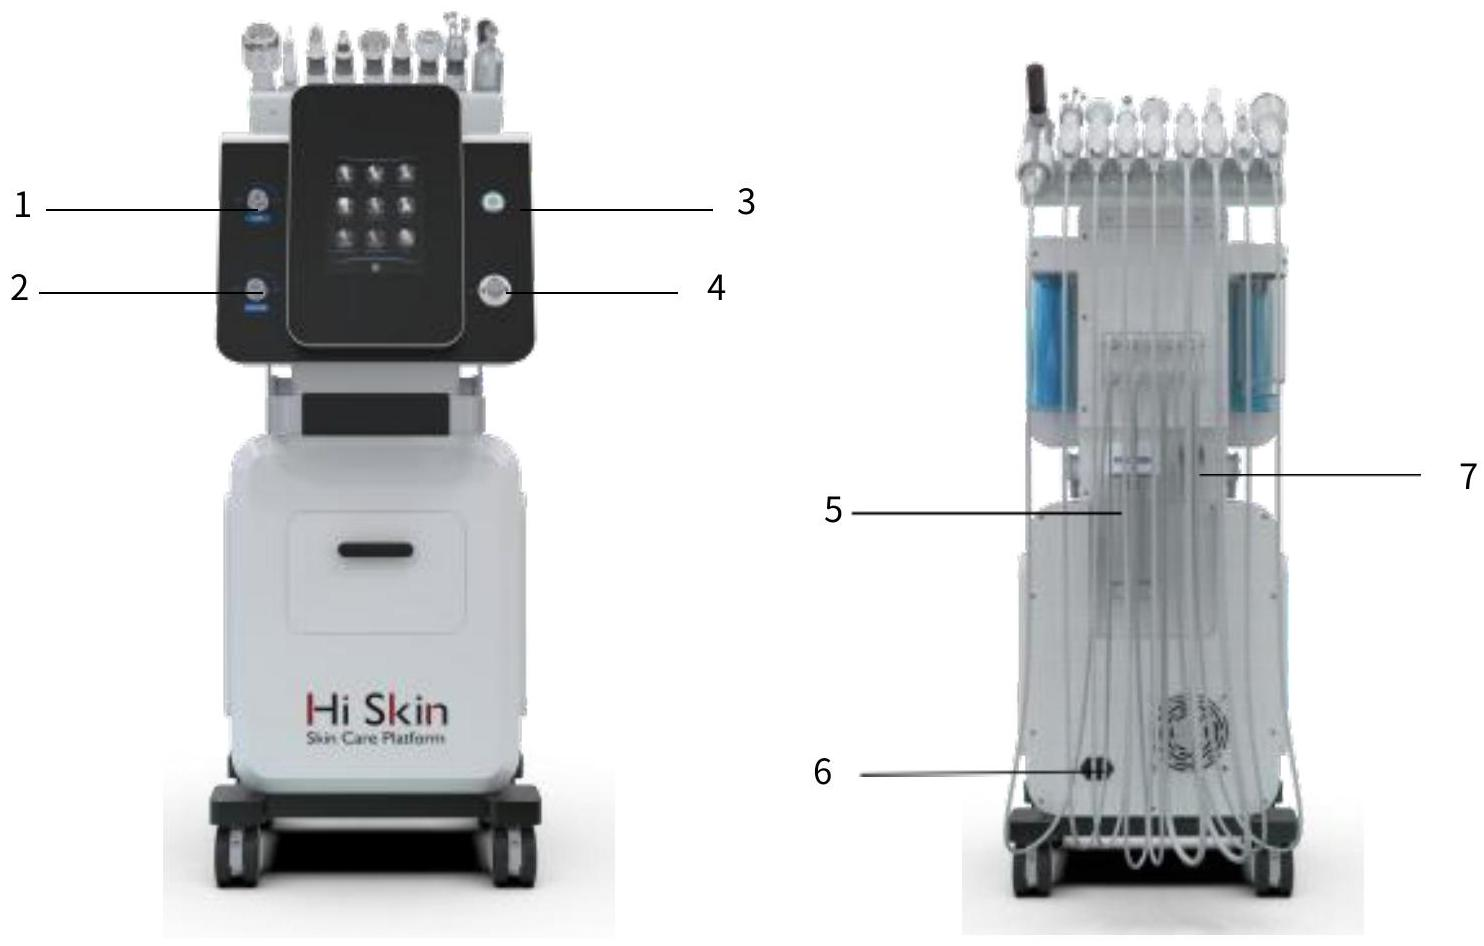
\includegraphics[width=\textwidth]{62504995-9f9b-47e6-9021-a213c68ce0b6-06_946_1484_651_214}
	\caption{}
\end{figure}

\begin{figure}[H]
	\centering
	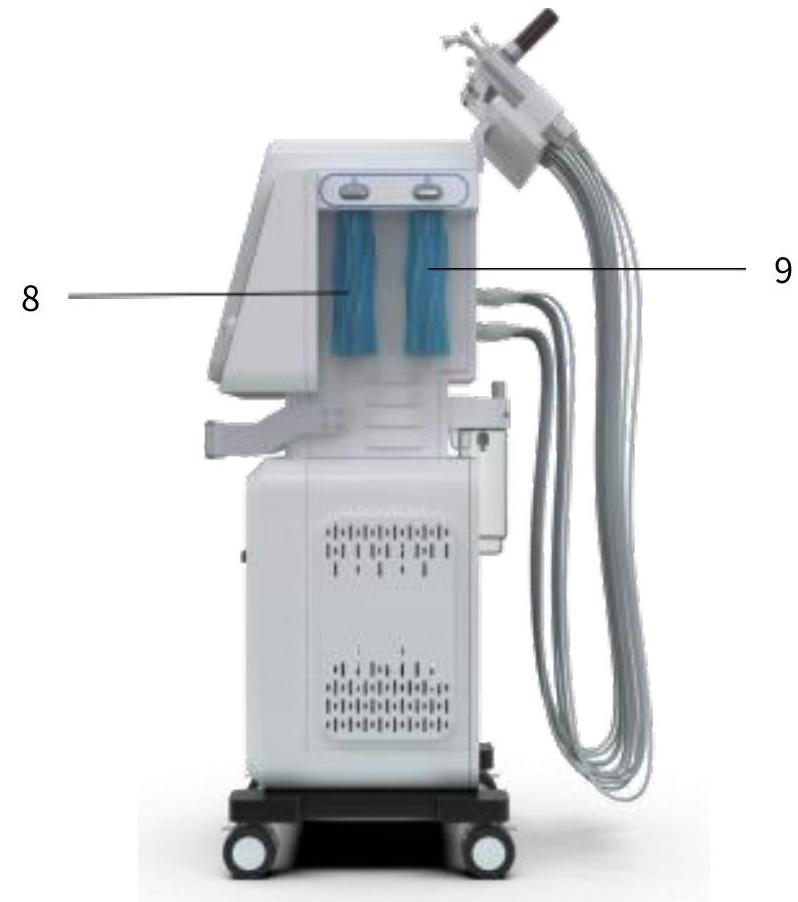
\includegraphics[width=\textwidth]{62504995-9f9b-47e6-9021-a213c68ce0b6-06_902_798_1774_221}
	\caption{}
\end{figure}

\begin{figure}[H]
	\centering
	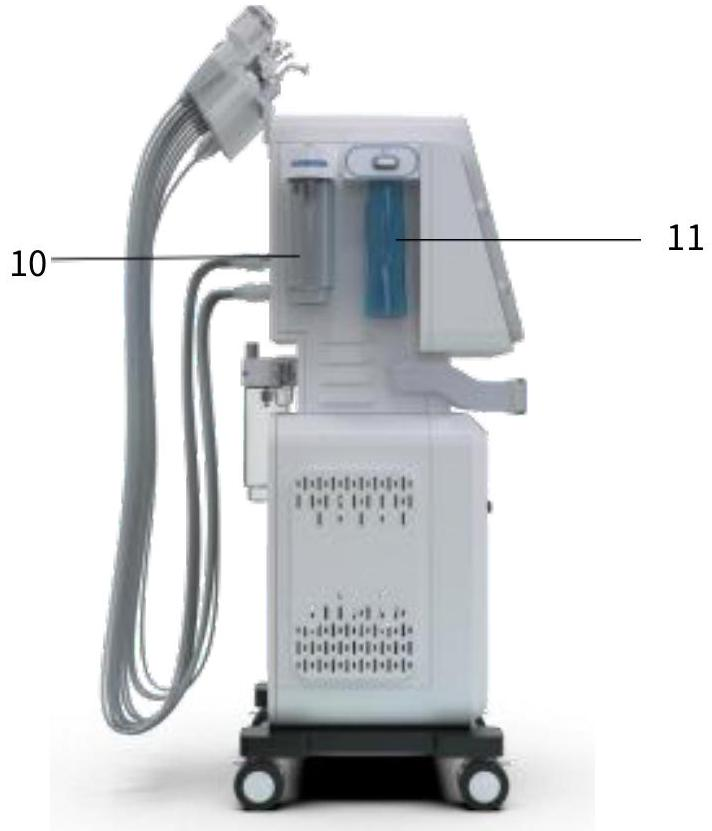
\includegraphics[width=\textwidth]{62504995-9f9b-47e6-9021-a213c68ce0b6-06_831_712_1845_1082}
	\caption{}
\end{figure}

\begin{table}[H]
	\centering
	\begin{tabularx}{\textwidth}{|X|X|}
		\hline
		\multicolumn{2}{|c|}{\textbf{Elenco dei componenti}} \\
		\hline
		\begin{minipage}[t]{\linewidth}
			\begin{enumerate}[leftmargin=*, itemsep=0pt, parsep=0pt, topsep=0pt, partopsep=0pt]
				\item Interruttore dell'aria
				\item Interruttore della quantità d'acqua
				\item Pulsante di attivazione/disattivazione
				\item Interruttore di selezione della bottiglia
				\item Bottiglia per l'acqua di scarico
				\item Connettore di alimentazione
				\item Filtro
			\end{enumerate}
		\end{minipage} &
		\begin{minipage}[t]{\linewidth}
			\begin{enumerate}[start=8, leftmargin=*, itemsep=0pt, parsep=0pt, topsep=0pt, partopsep=0pt]
				\item Bottiglia
				\item Bottiglia B
				\item Bottiglia di acqua di scarico per bolle di schiuma
				\item Bottiglia C
			\end{enumerate}
		\end{minipage} \\
		\hline
	\end{tabularx}
\end{table}

\subsection{Funzione delle bottiglie A, B, C}
\begin{itemize}
  \item A: Essenza detergente profonda. Viene utilizzata per una pulizia profonda della pelle. Azionando l'impugnatura, può assorbire e rimuovere le impurità dalla pelle.
  \item B: Essenza di acqua vitale ed ossigeno. Idrata dopo la detersione, schiarendo e idratando la pelle.
  \item C: Soluzione detergente con acqua e ossigeno. Utilizzata per pulire il tubo dell'impugnatura dell'utensile.
\end{itemize}

\section{Proporzione della soluzione madre:}
Il flacone con i concentrati A, B, C corrisponde al flacone A, B, C sul dispositivo. Versare prima la soluzione madre nel flacone corrispondente, aggiungere acqua pulita in un rapporto di 1:40 e agitare bene, quindi rabboccare con acqua pulita. La durata di conservazione della soluzione madre preparata è di 7 giorni.

Nota:Quando l'intera bottiglia di diluente è esaurita, l'acqua calda nelle bottiglie A, B, C deve essere pulita di nuovo nello stesso modo del tubo del mulino ad acqua per evitare che il tubo si ostruisca.

\subsection{Maniglie e funzioni attrezzate}
\subsection{Manipolo per idrodermoabrasione}

Apre i pori, ammorbidisce lo strato corneo, pulisce la pelle in profondità, idrata in profondità, rimuove i punti neri, migliora la pelle giallo scuro e rende la pelle pulita, bianca ed elastica.\\

\begin{figure}[H]
	\centering
	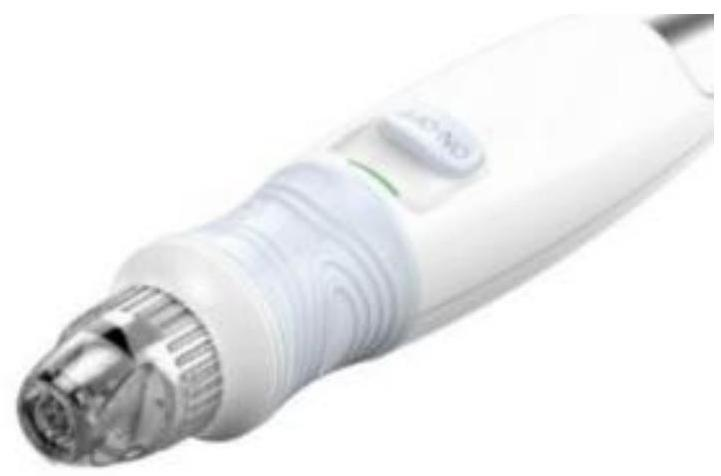
\includegraphics[width=0.7\linewidth]{62504995-9f9b-47e6-9021-a213c68ce0b6-07_476_721_1761_1233}
\end{figure}

Grazie alle diverse testine di trattamento, gli utenti possono scegliere la testina di trattamento più adatta alle proprie esigenze in base alle condizioni della pelle.\\

\begin{figure}[H]
	\centering
	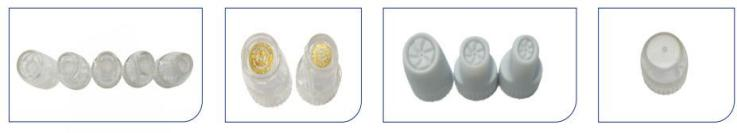
\includegraphics[width=\linewidth, height=\textheight, keepaspectratio]{User manual .sk.it.pdf-image-024.jpg}
	\caption{Testina di pulizia idraulica rigida, Testina per microdermoabrasione, Testina di pulizia in silicone morbido, Testina per la pulizia dei tubi}
	\label{}
\end{figure}


\subsection{Cold Hammer (manipolo caldo/freddo)}
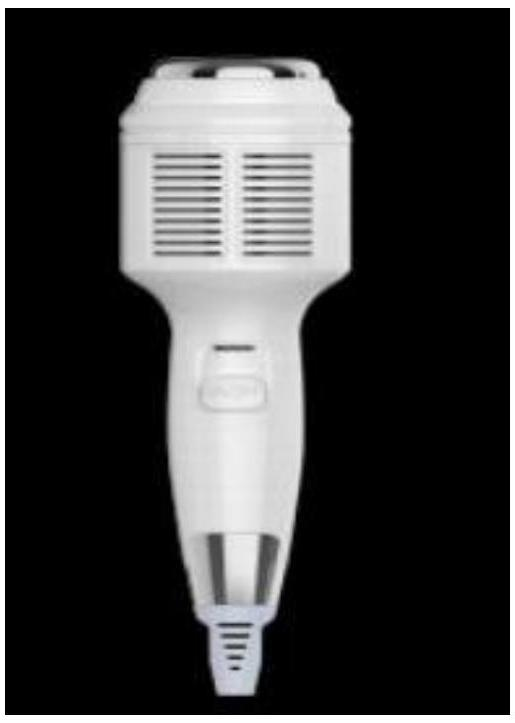
\includegraphics[max width=\textwidth, alt={}, center]{62504995-9f9b-47e6-9021-a213c68ce0b6-08_723_515_840_123}

Cold Hammer $0^{\circ} \mathrm{C}$ : Ghiaccia la pelle, restringe i pori, lenisce la pelle.

Hot hammer $45^{\circ} \mathrm{C}$ : aumenta la temperatura superficiale della pelle, accelera la circolazione sanguigna e aumenta il tasso di assorbimento se utilizzato con prodotti cosmetici

\subsection{Manipolo spray polimerico}

Quando combinato con prodotti liquidi, il liquido si trasforma in piccole molecole simili a nebbia mediante atomizzazione ad alta pressione e successiva spruzzatura ad alta pressione su ottenere un effetto idratante profondo.\\
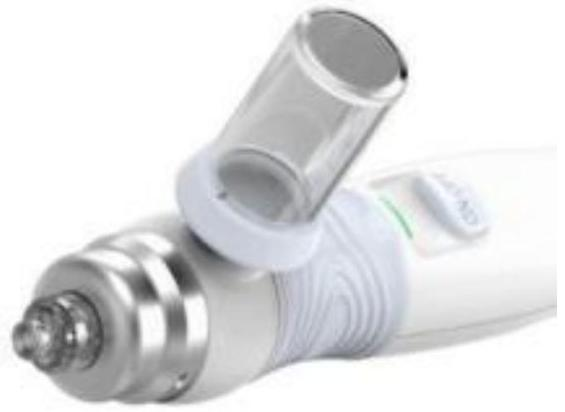
\includegraphics[max width=\textwidth, alt={}, center]{62504995-9f9b-47e6-9021-a213c68ce0b6-08_412_565_1923_1411}


\subsection{Manipolo a ultrasuoni}

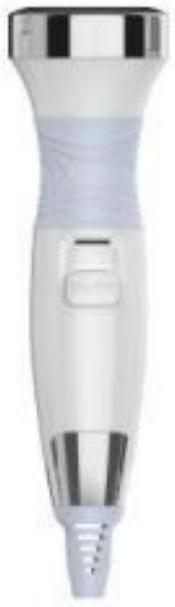
\includegraphics[max width=\textwidth, alt={}, center]{62504995-9f9b-47e6-9021-a213c68ce0b6-09_607_175_376_415}

A una frequenza da 1 milione a 3 milioni di vibrazioni al secondo, rapidamente apre i pori e permette all'essenza di penetrare nello strato basale pelle.

\subsection{Manipolo RF (radiofrequenza) bipolare}

Il trattamento RF è un metodo non invasivo per ottenere il rassodamento della pelle e raggiungere aspetto più giovane. L'energia RF riscalda in profondità gli strati della pelle (derma) del tuo corpo per produrre\\
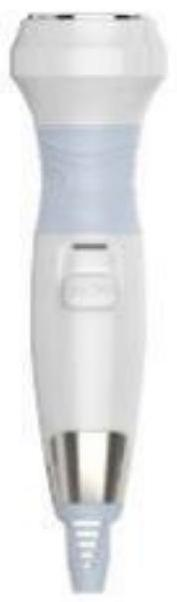
\includegraphics[max width=\textwidth, alt={}, center]{62504995-9f9b-47e6-9021-a213c68ce0b6-09_602_177_1231_1425}\\
collagene.

\subsection{Manipolo per schiuma ossigenante (mousse)}

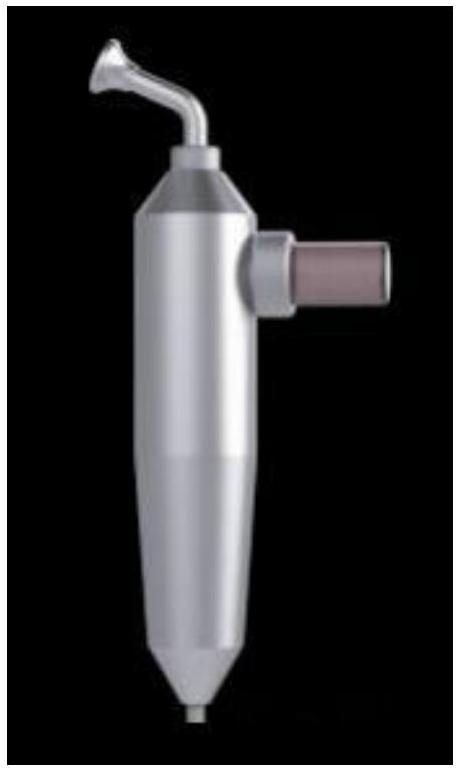
\includegraphics[max width=\textwidth, alt={}, center]{62504995-9f9b-47e6-9021-a213c68ce0b6-10_768_456_324_255}

L'impugnatura crea una schiuma densa contenente una grande quantità componenti dell'ossigeno attivo. Grazie alle elevate proprietà ossidanti dell'ossigeno attivo, gli ioni idrossido possono penetrare rapidamente nella pelle, ottenendo l'effetto di pulizia, idratazione e ringiovanimento della pelle.

\subsection{Manipolo vibrante a ultrasuoni per la pulizia della pelle}

Rimuovere morto pelle alta frequenza\\
Le onde vibranti rimuovono i punti neri, ammorbidiscono i cheratinociti della pelle e purificano in profondità le impurità dalla pelle.\\
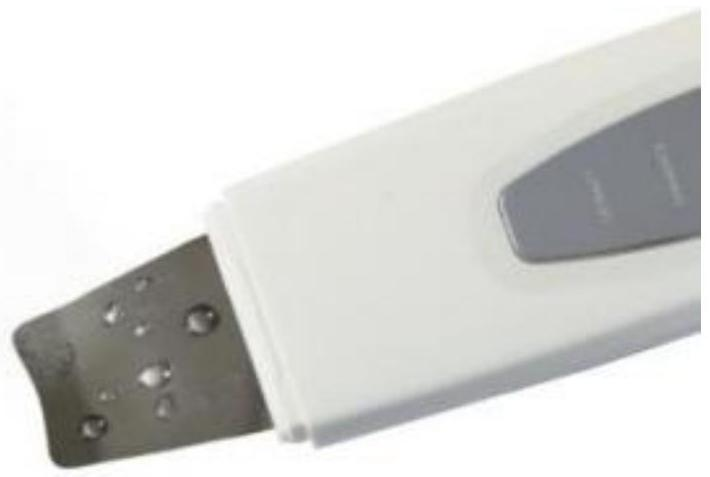
\includegraphics[max width=\textwidth, alt={}, center]{62504995-9f9b-47e6-9021-a213c68ce0b6-10_477_710_1573_1292}

\subsection{Manipolo a microcorrenti}

\begin{figure}[H]
	\centering
	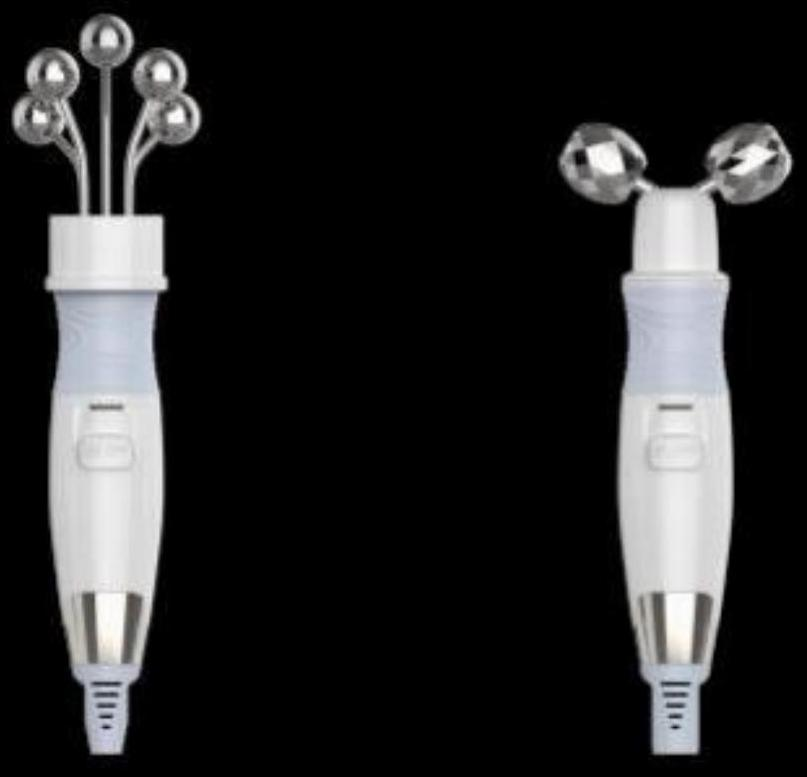
\includegraphics[width=0.7\linewidth]{62504995-9f9b-47e6-9021-a213c68ce0b6-11_777_807_317_169}
	\caption{La microcorrente utilizza l'elettricità a bassa tensione per stimolazione muscolare e produzione di adenosina crescita cellulare del trifosfato (ATP) e rigenerazione del collagene nel derma del viso.}
\end{figure}





\section{Sicurezza e conformità}
\subsection{Sicurezza del cliente}
La sicurezza del cliente dipende principalmente dalla formazione degli operatori, dalla consulenza del cliente, da un'analisi adeguata della pelle e da una sala trattamenti adeguata. Gli operatori devono informare il cliente di tutti i rischi associati all'uso di questa apparecchiatura.

\subsection{Precauzioni di sicurezza}
\subsubsection{Precauzioni di sicurezza nel punto di utilizzo}
\begin{itemize}
  \item L'uso di cavi di alimentazione danneggiati o manomessi può causare incendi e scosse elettriche. attuale;
  \item Non piegare o scuotere eccessivamente il cavo di alimentazione per evitare incendi e scosse elettriche.
  \item Se l'utensile è allentato o danneggiato, contattare tempestivamente l'azienda.
  \item Non utilizzare il dispositivo in un ambiente instabile, ad esempio in caso di inclinazione, spostamento o impatto;
  \item Non deve esserci acqua o sporcizia all'interno del dispositivo. Se entrano oggetti estranei, contattare l'azienda in tempo;
  \item L'utensile deve essere scollegato prima di spostarlo; Quando l'utensile è in movimento, evitare vibrazioni della macchina;
  \item Il dispositivo deve essere posizionato in un luogo stabile e deve lasciare circa 5 cm di spazio per Assicurare la circolazione dell'aria e facilitare la dissipazione del calore;
  \item Non coprire nulla sul dispositivo per evitare che i fori di ventilazione vengano bloccati;
  \item Evitare di utilizzare il dispositivo nei seguenti ambienti: esposizione alla luce solare; ambiente con elevata umidità; ambiente vicino all'acqua; vibrazioni, luogo di inclinazione; ambiente con forte campo magnetico; luogo di verificarsi di onde elettromagnetiche, sovratensioni; luogo di stoccaggio di sostanze chimiche; ambiente con gas corrosivo;
  \item Questo dispositivo deve essere posizionato lontano da radio, televisori, fotocopiatrici, fax, ecc.;
  \item Non utilizzarlo con altri elettrodomestici (come il forno a microonde) per evitare interferenze tra\\
strumenti e non ha causato alcun malfunzionamento.
\end{itemize}

\subsubsection{Precauzioni prima dell'uso}
\begin{itemize}
  \item Leggere attentamente il manuale operativo prima di avviare la macchina. L'operatore deve avere familiarità con le istruzioni per l'uso e il metodo operativo. Lo strumento deve essere gestito\\
professionisti;\\
L'impostazione dei parametri operativi deve essere effettuata sotto la guida di un esperto; Prima dell'uso verificare se il dispositivo funziona normalmente;
  \item Assicurarsi che il filo di terra sia collegato correttamente; Controllare che tutti i fili siano correttamente connesso e protetto;
  \item Quando si utilizza l'utensile, assicurarsi di utilizzarlo correttamente. In caso contrario, potrebbero verificarsi incidenti. pericoli e bisogna prestarvi attenzione.
\end{itemize}

\subsubsection{Precauzioni di sicurezza durante l'uso}
\begin{itemize}
  \item Quando si verifica una situazione anomala durante il funzionamento dello strumento o del paziente, l'operatore deve immediatamente lasciare la maniglia di controllo fuori dal paziente e premere l'interruttore di alimentazione per interrompere l'uso dello strumento;
  \item Durante il funzionamento del dispositivo, è necessario monitorare costantemente la situazione degli ospiti e del dispositivo e prestare attenzione a eventuali situazioni anomale che si verificano in qualsiasi momento;\\
\$Il dispositivo deve essere utilizzato correttamente da un operatore qualificato.
\end{itemize}

\subsubsection{Precauzioni post-uso}
\begin{itemize}
  \item Una volta completata l'operazione, la leva di comando ritorna alla cerniera della leva di comando.
  \item Dopo aver utilizzato la maniglia di controllo, è necessario pulire la sonda prima di utilizzarla nuovamente.
\end{itemize}

\subsection{Sicurezza elettrica}
Per garantire un utilizzo sicuro, la tensione di esercizio nominale del sistema è di 220 V , la corrente di ingresso massima è di 10 A o 110 V e la corrente di ingresso massima è di 15 A .

\section{Procedura di installazione}
Il processo di installazione include:

\begin{itemize}
  \item Disimballare il dispositivo e controllarne il contenuto.
  \item Preparare una soluzione madre.
  \item Installare le bottiglie A, B, C e due bottiglie per l'acqua di scarico.
  \item Collegare l'alimentatore.
  \item Accendere e testare tutte le funzioni/parametri del sistema.
\end{itemize}

\subsection{Elenco degli accessori}
\begin{center}
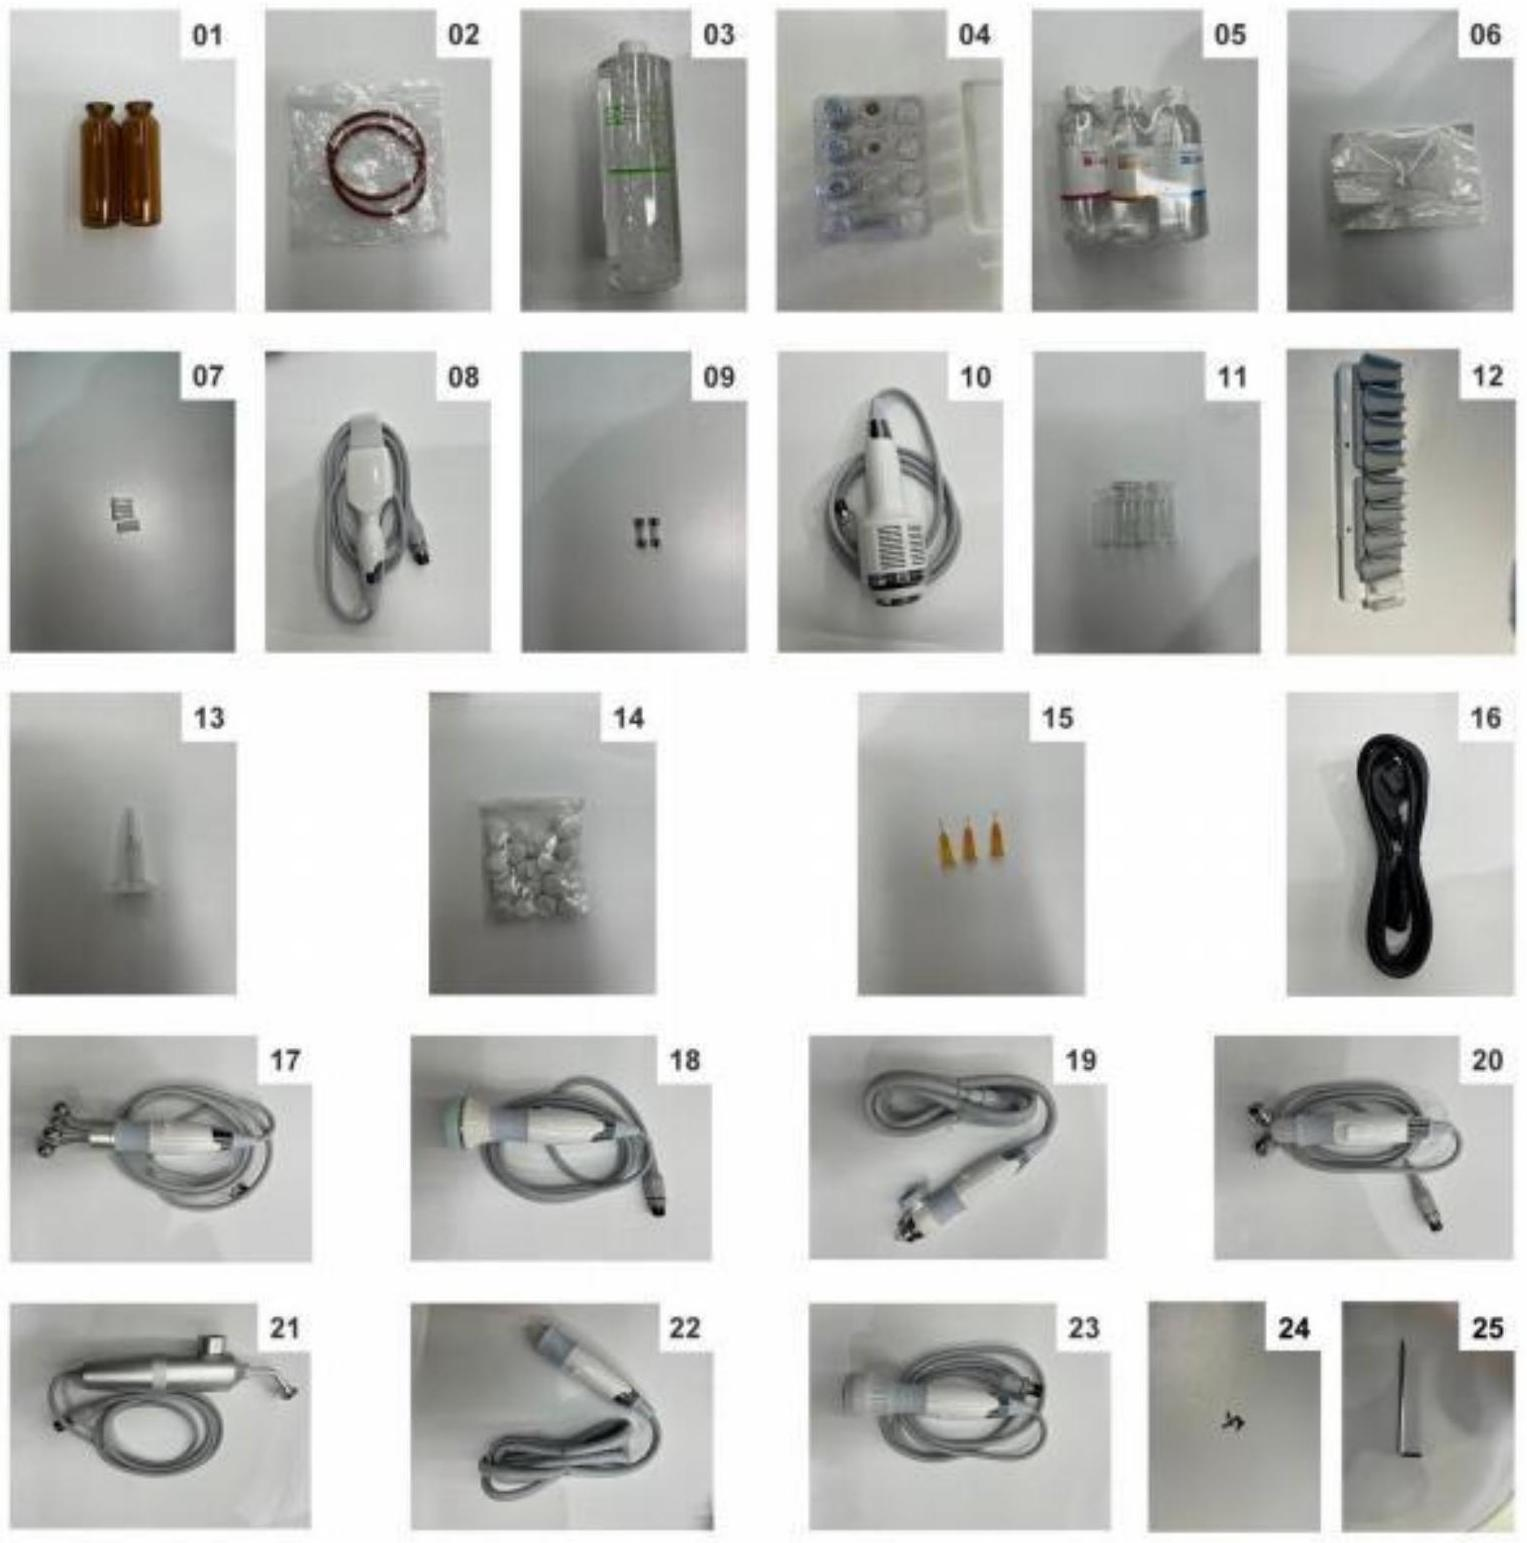
\includegraphics[max width=\textwidth, alt={}]{62504995-9f9b-47e6-9021-a213c68ce0b6-14_1543_1527_877_269}
\end{center}

\begin{table}[H]
	\centering
	\begin{tabular}{|p{4.5cm}|p{4.5cm}|p{4.5cm}|}
		\hline
		1. Bottiglia di schiuma & 9. Fusibile & 17. Multipolare maniglia microcorrente \\
%		\hline
		2. Anello di gomma & 10. Freddo maniglia martelli & 18. Handle di importazione degli ultrasuoni \\
%		\hline
		3. Acqua frizzante & 11. Bottiglia con spray maniglia & 19. Impugnatura spray polimerica \\
%		\hline
		4. Testine per dermoabrasione & 12. Supporto per maniglia & 20. Manico microcorrente bipolare \\
%		\hline
		5. Soluzione madre & 13. Ugello spray per la pulizia dell'ago & 21. Maniglia in schiuma a bolle \\
%		\hline
		6. Testa di trattamento spray & 14. Fogli di schiuma di cotone a bolle maniglia & 22. Manico per idrodermoabrasione \\
%		\hline
		7. Filtri con maniglia a bolle di schiuma & 15. Maniglia in schiuma a bolle & 23. RF bipolare maniglia \\
%		\hline
		8. Maniglia a vibrazione ultrasonica & 16. Cavo di alimentazione & 24. Viti \\
%		\hline
		&  & 25. Cacciavite \\
		\hline
	\end{tabular}
\end{table}

\subsection{L'installazione è importante, utilizzare il dispositivo rispettando i seguenti requisiti:}
\begin{itemize}
  \item Temperatura ambiente di lavorazione: $10^{\circ} \mathrm{C} \sim 30^{\circ} \mathrm{C}$
  \item Umidità relativa: $\leqslant 75 \%$
  \item Pressione dell'aria: 860-1060 hpa
  \item Requisiti di alimentazione: CA $220 \mathrm{~V} \pm 10 \% ; 50 \mathrm{~Hz} \pm 2\%$
\end{itemize}

\begin{itemize}
  \item Acqua: acqua pura
\end{itemize}

\subsection{Installare i cilindri A, B e C}
\begin{itemize}
  \item Utilizzare la soluzione madre di essenza di ossigeno destinata al dispositivo.
  \item Installazione della bottiglia: sono disponibili le soluzioni A, B, C e due bottiglie di scarico, installarle secondo quanto sopra marche:\\
  
\begin{figure}[H]
	\centering
	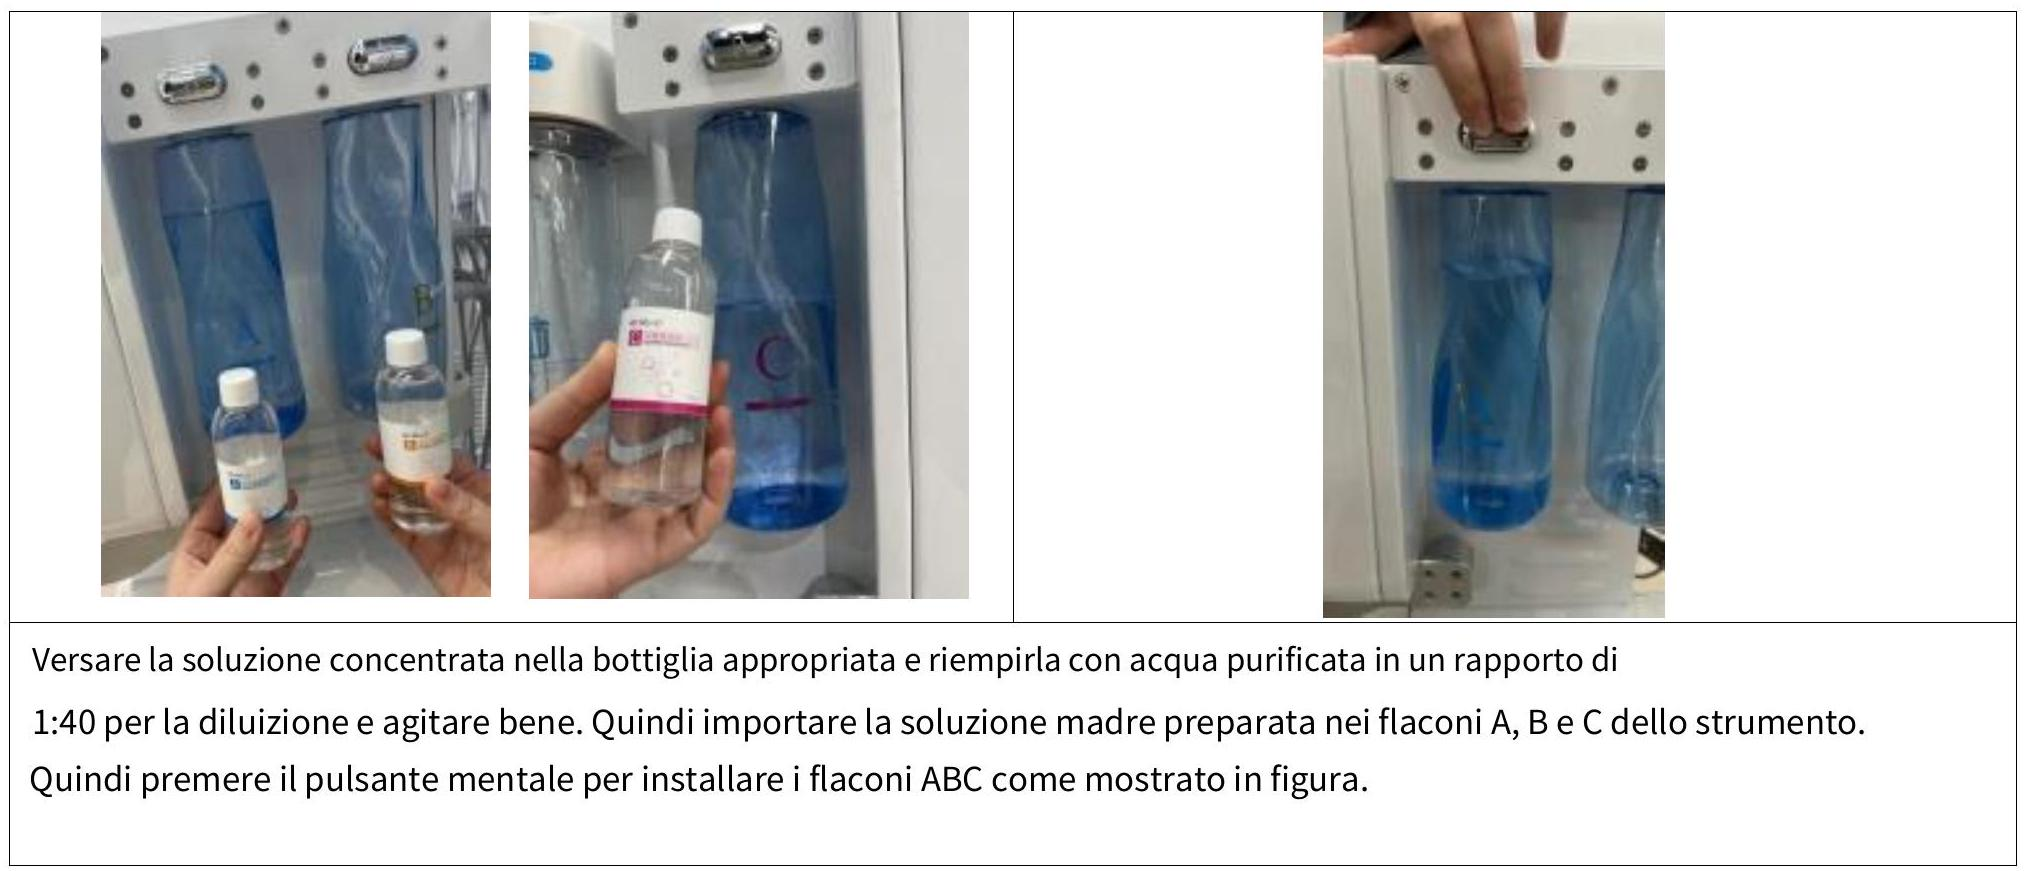
\includegraphics[width=\textwidth]{62504995-9f9b-47e6-9021-a213c68ce0b6-15_871_2025_1836_20}
%	\caption{}
\end{figure}

\begin{figure}[H]
	\centering
	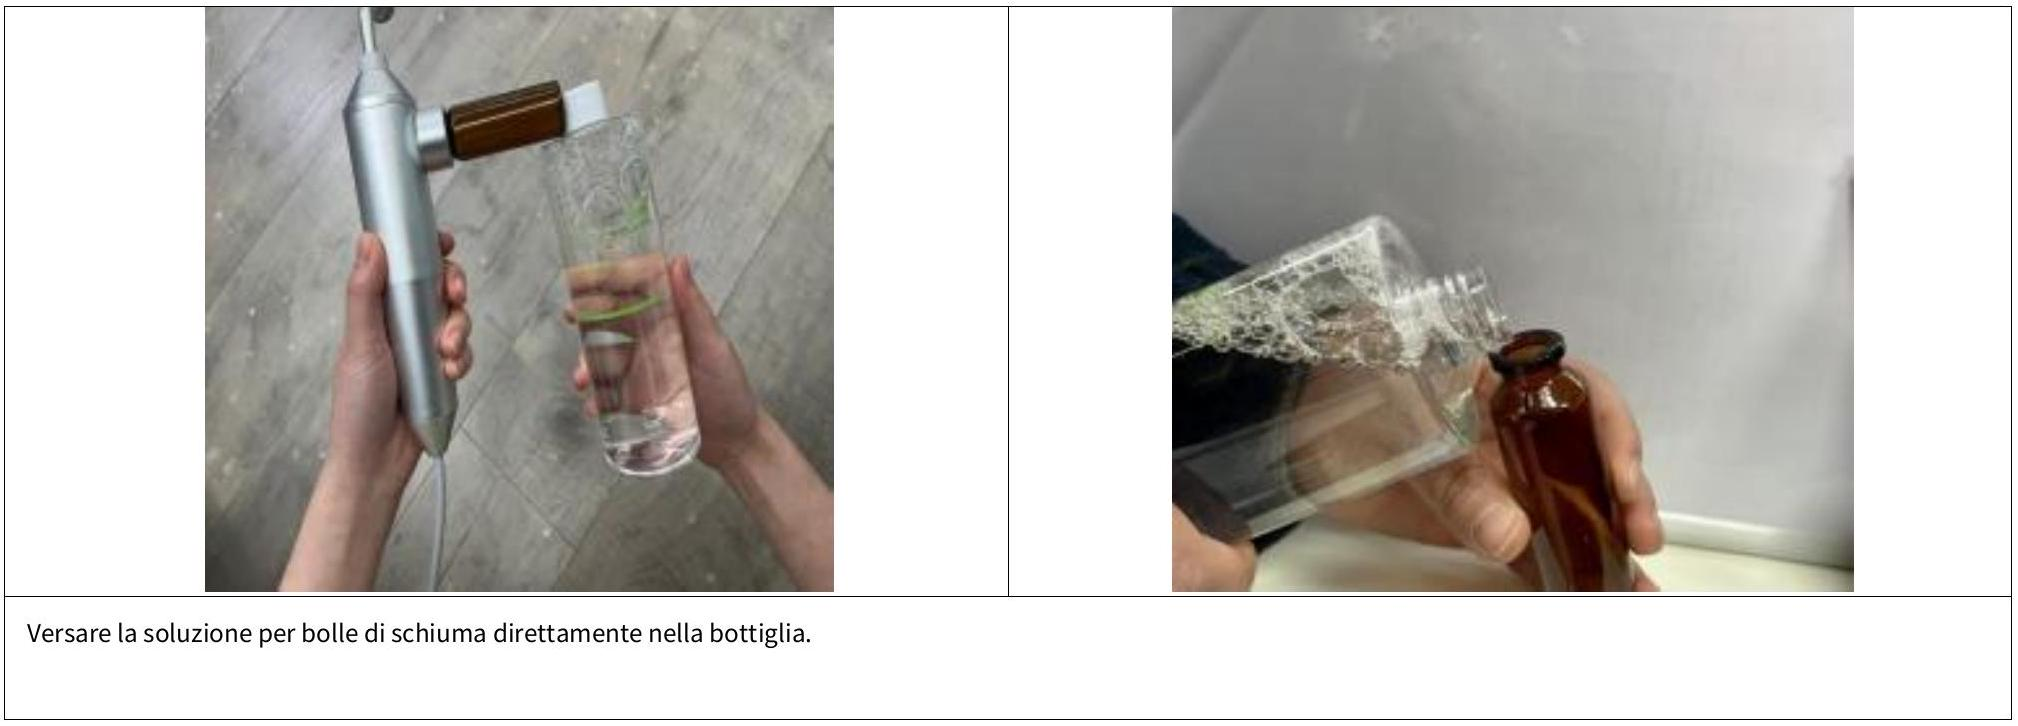
\includegraphics[width=\textwidth]{62504995-9f9b-47e6-9021-a213c68ce0b6-16_726_2018_191_25}
%	\caption{}
\end{figure}

\begin{figure}[H]
	\centering
	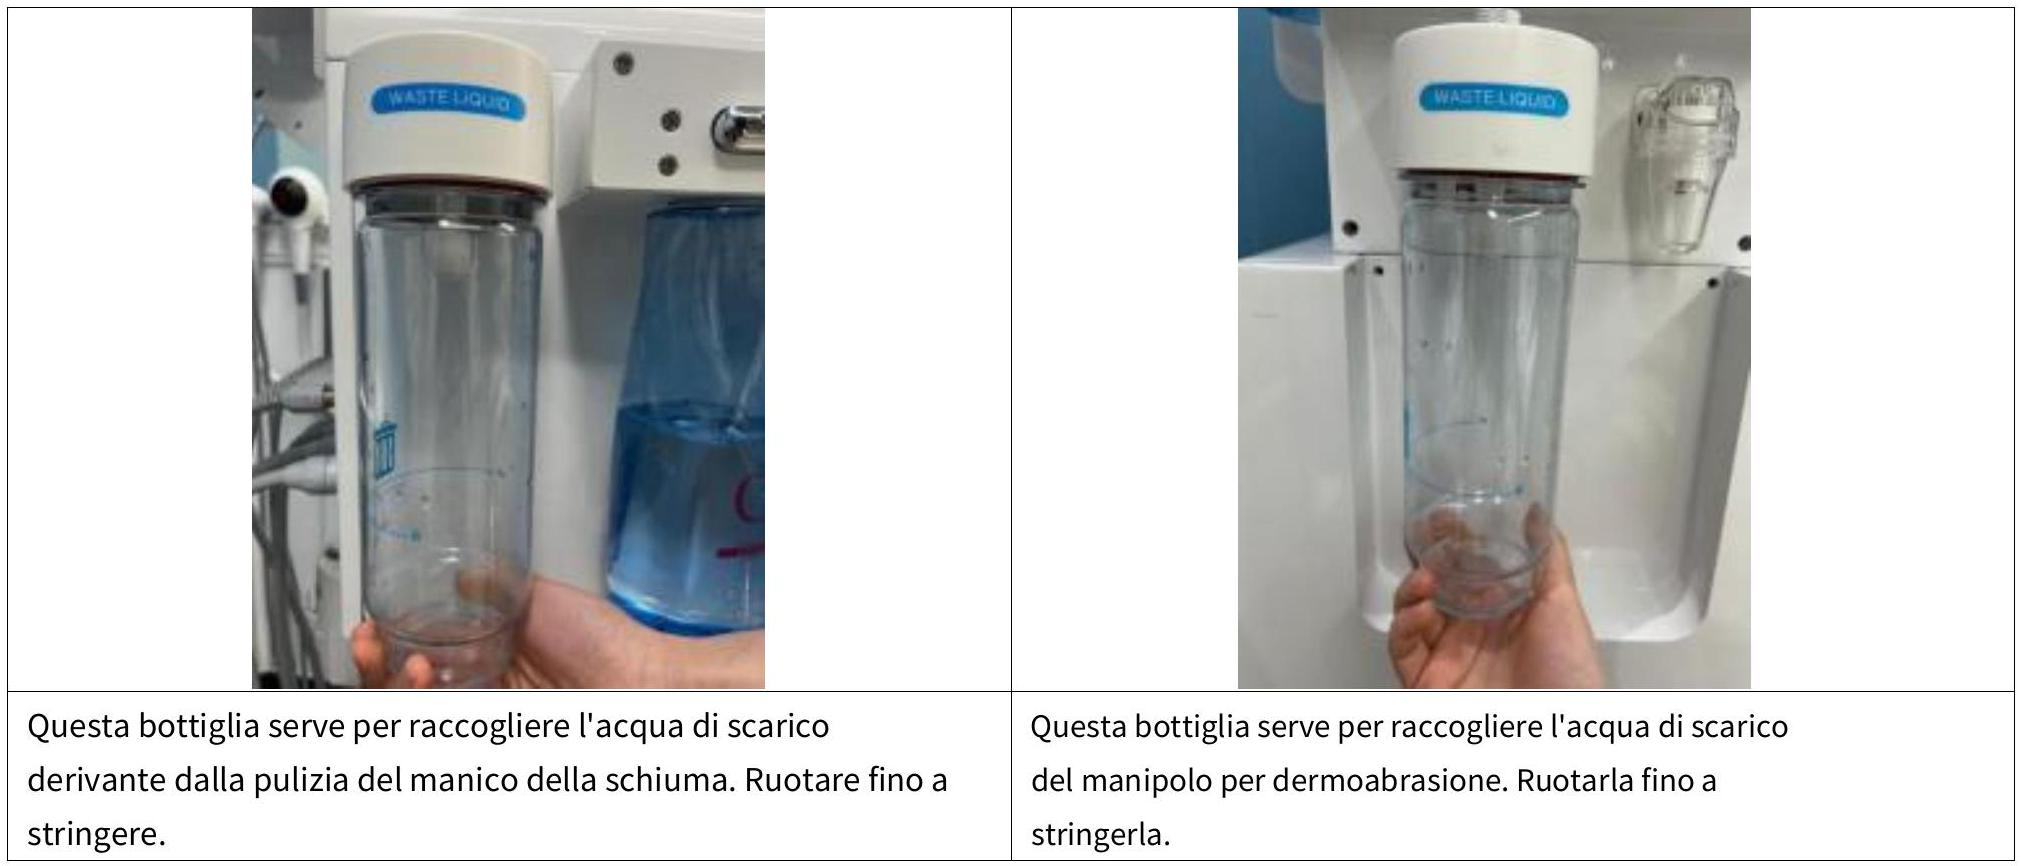
\includegraphics[width=\textwidth]{62504995-9f9b-47e6-9021-a213c68ce0b6-16_866_2021_964_22}
	%	\caption{}
\end{figure}
\end{itemize}

\subsection{Installare le staffe della maniglia}

\begin{figure}[H]
	\centering
	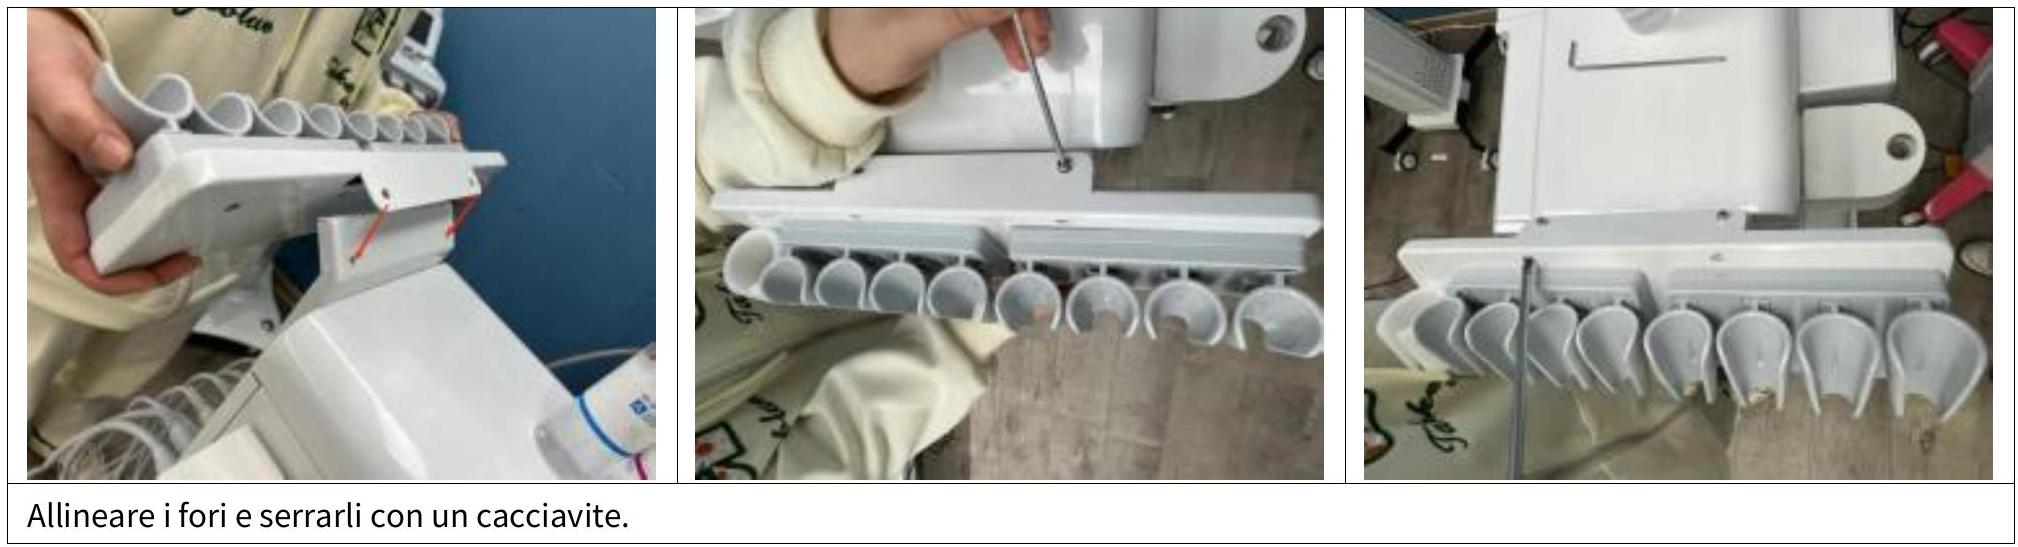
\includegraphics[width=\textwidth]{62504995-9f9b-47e6-9021-a213c68ce0b6-16_547_2018_1955_22}
	%	\caption{}
\end{figure}

\subsection{Installare la maniglia}
Impugnatura microcorrente bipolare: collegare il cavo e girare la manopola mentale.\\
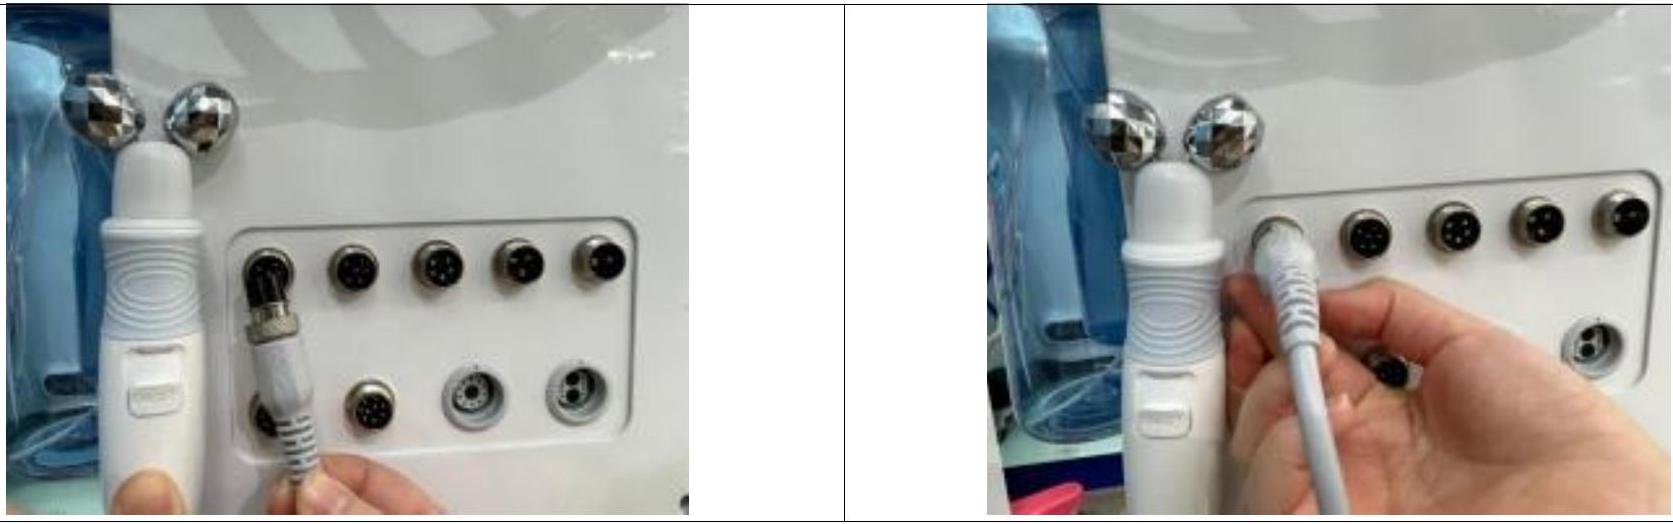
\includegraphics[max width=\textwidth, alt={}, center]{62504995-9f9b-47e6-9021-a213c68ce0b6-17_524_1673_324_189}

Maniglia di importazione degli ultrasuoni: collegare il cavo e girare la manopola mentale.\\
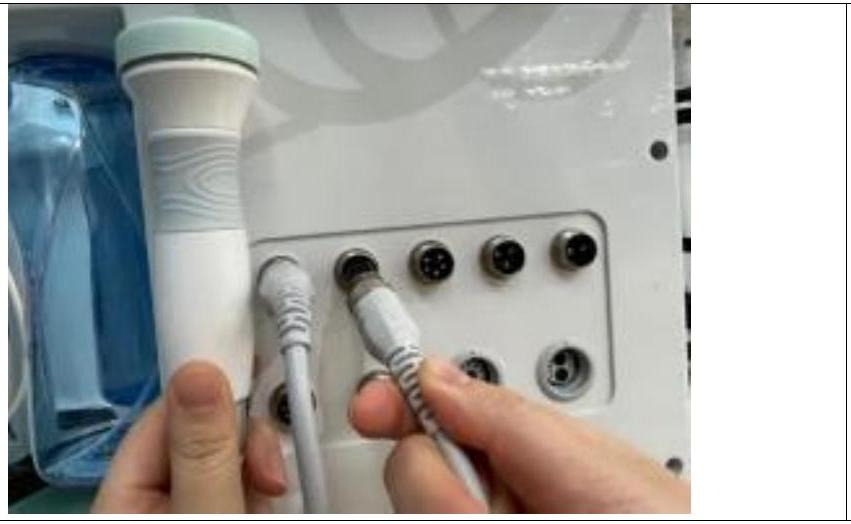
\includegraphics[max width=\textwidth, alt={}, center]{62504995-9f9b-47e6-9021-a213c68ce0b6-17_524_851_904_187}\\
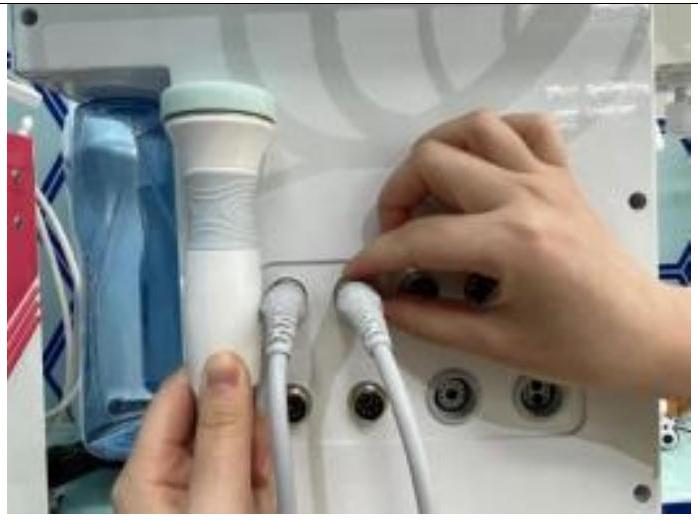
\includegraphics[max width=\textwidth, alt={}, center]{62504995-9f9b-47e6-9021-a213c68ce0b6-17_520_698_904_1169}

Impugnatura microcorrente multipolare: collegare il cavo e ruotare la manopola mentale.\\
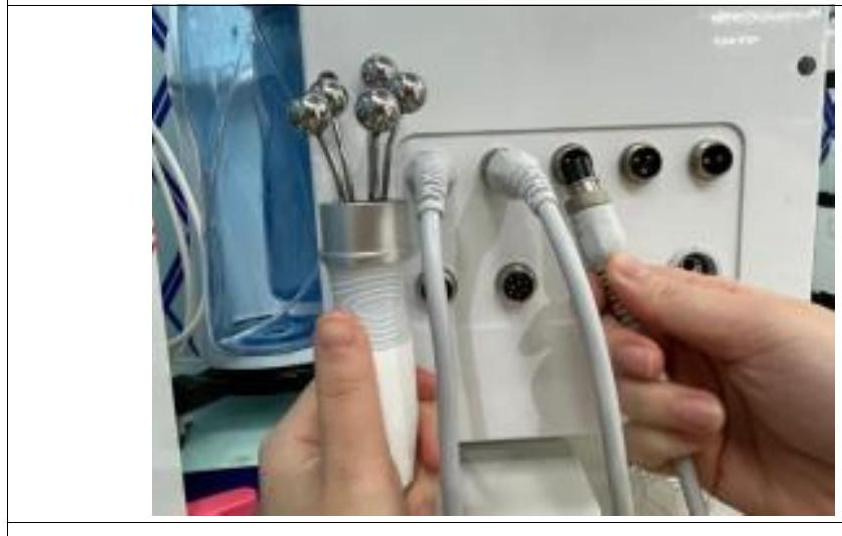
\includegraphics[max width=\textwidth, alt={}, center]{62504995-9f9b-47e6-9021-a213c68ce0b6-17_536_842_1530_22}\\
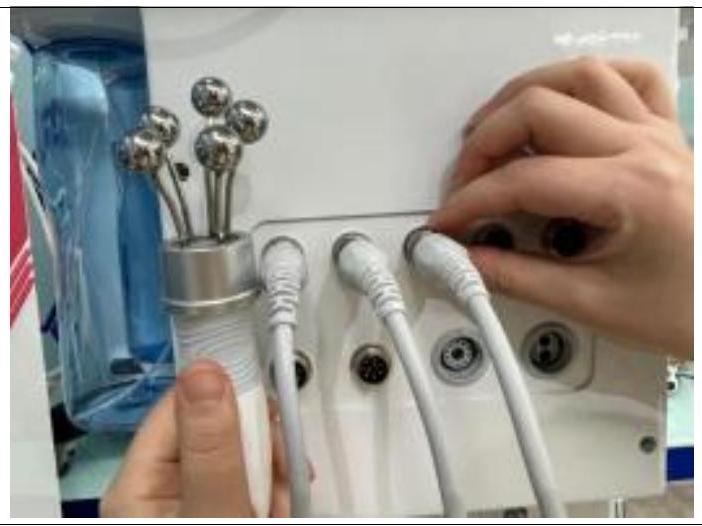
\includegraphics[max width=\textwidth, alt={}, center]{62504995-9f9b-47e6-9021-a213c68ce0b6-17_526_702_1528_1169}

Impugnatura vibrante a ultrasuoni: collegare il cavo e girare la manopola.\\
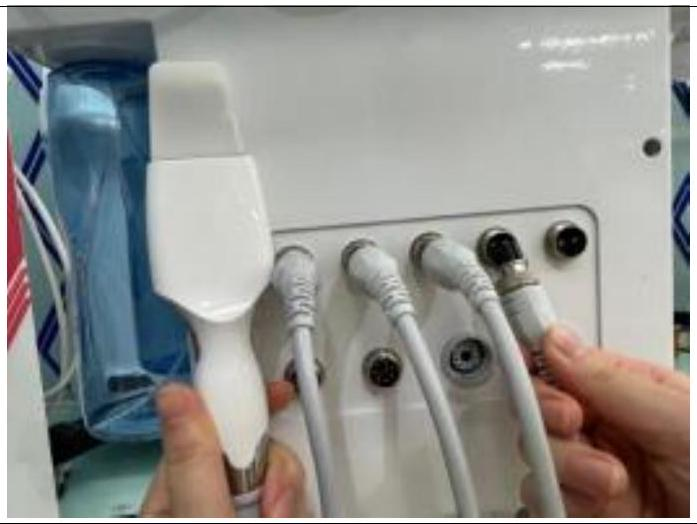
\includegraphics[max width=\textwidth, alt={}, center]{62504995-9f9b-47e6-9021-a213c68ce0b6-17_524_697_2156_169}\\
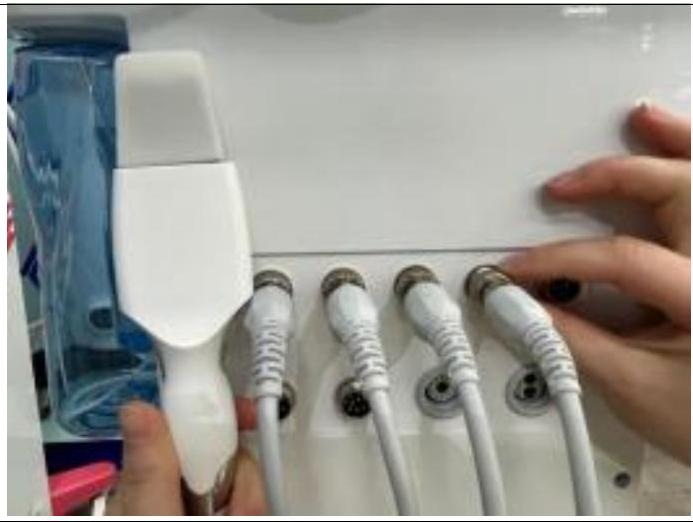
\includegraphics[max width=\textwidth, alt={}, center]{62504995-9f9b-47e6-9021-a213c68ce0b6-17_522_693_2158_1169}

\begin{figure}[H]
\begin{center}
\captionsetup{labelformat=empty}
\caption{Mousses Bubble Handle: collegare il cavo e girare la manopola mentale.}
  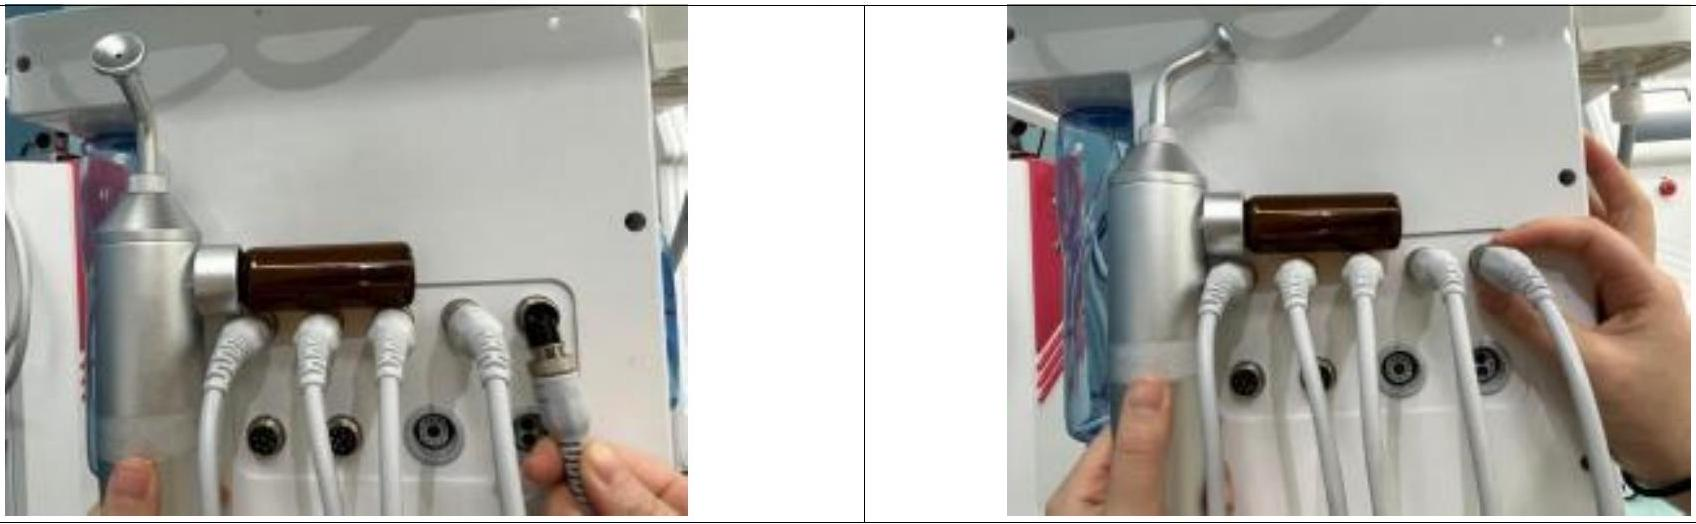
\includegraphics[alt={},max width=\textwidth]{62504995-9f9b-47e6-9021-a213c68ce0b6-18_524_1696_255_169}
\end{center}
\end{figure}

Impugnatura RF bipolare: collegare il cavo e ruotare la manopola mentale.\\
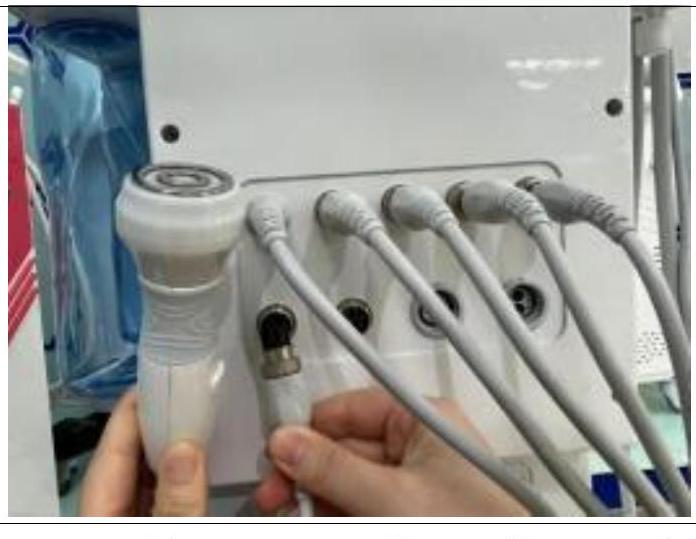
\includegraphics[max width=\textwidth, alt={}, center]{62504995-9f9b-47e6-9021-a213c68ce0b6-18_539_696_833_166}\\
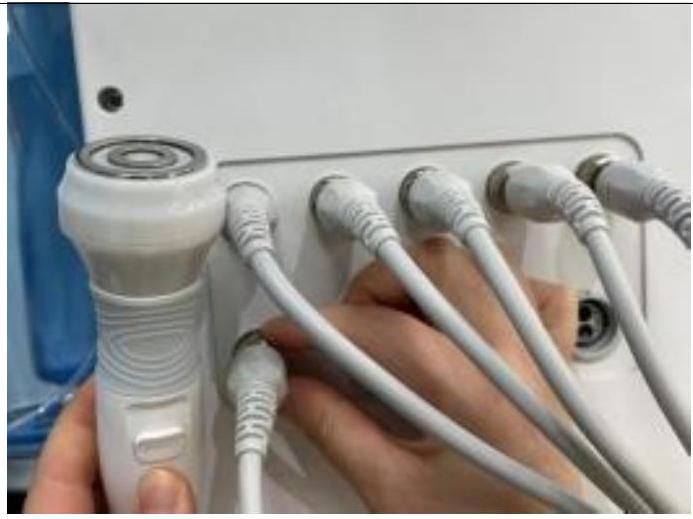
\includegraphics[max width=\textwidth, alt={}, center]{62504995-9f9b-47e6-9021-a213c68ce0b6-18_519_693_836_1169}

Impugnatura Cold Hammer: collegare il cavo e girare la manopola.\\
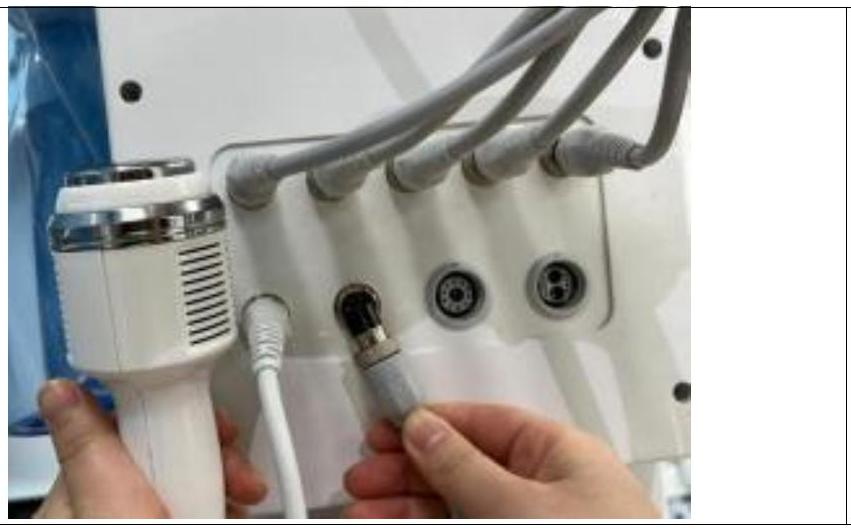
\includegraphics[max width=\textwidth, alt={}, center]{62504995-9f9b-47e6-9021-a213c68ce0b6-18_529_851_1411_187}\\
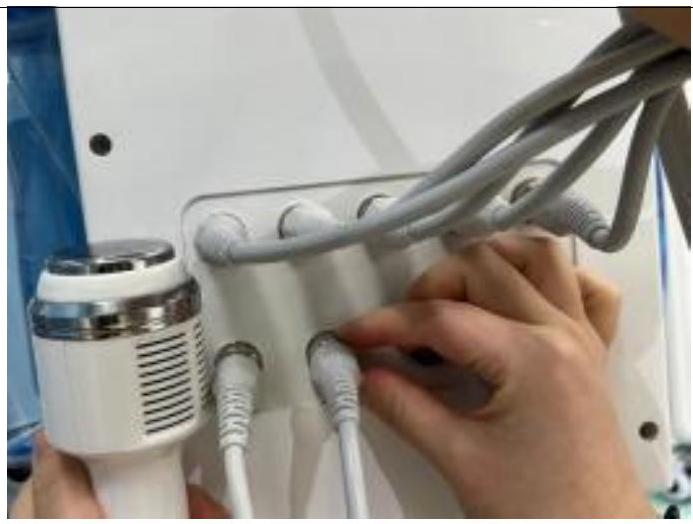
\includegraphics[max width=\textwidth, alt={}, center]{62504995-9f9b-47e6-9021-a213c68ce0b6-18_524_693_1411_1169}

Impugnatura dello spruzzatore polimerico: collegare il cavo.\\
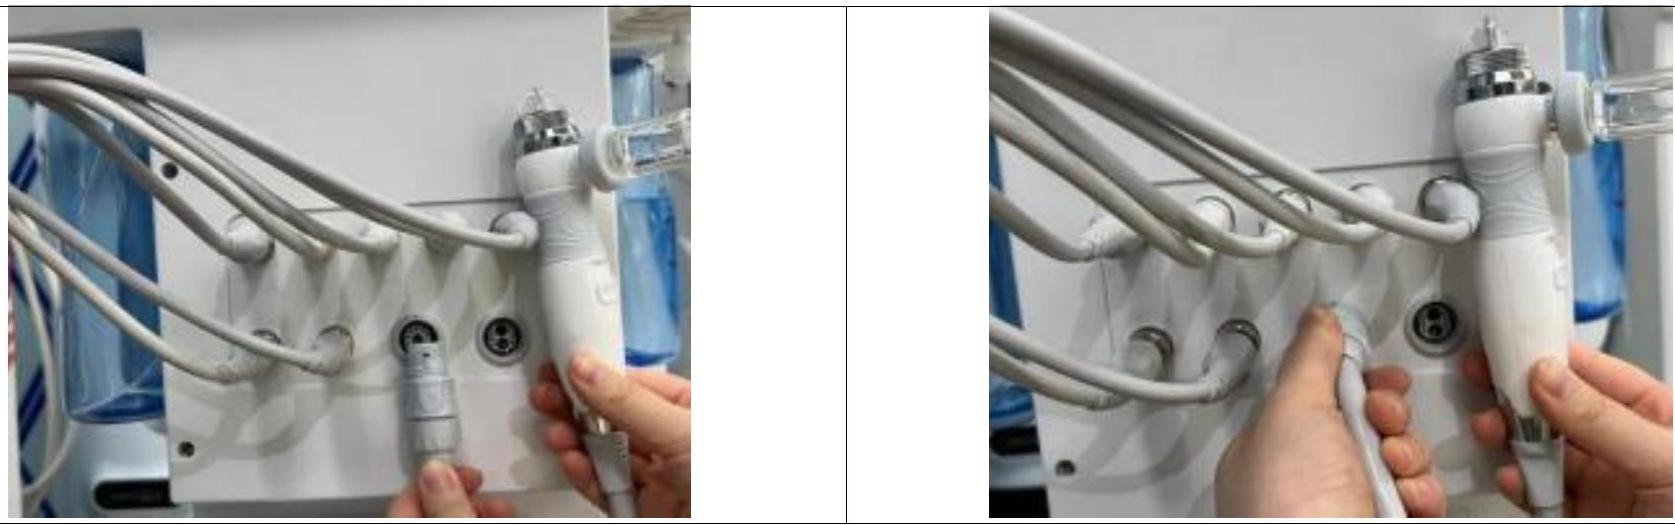
\includegraphics[max width=\textwidth, alt={}, center]{62504995-9f9b-47e6-9021-a213c68ce0b6-18_525_1675_1991_187}

Manico per idrodermoabrasione: collegare il cavo.\\
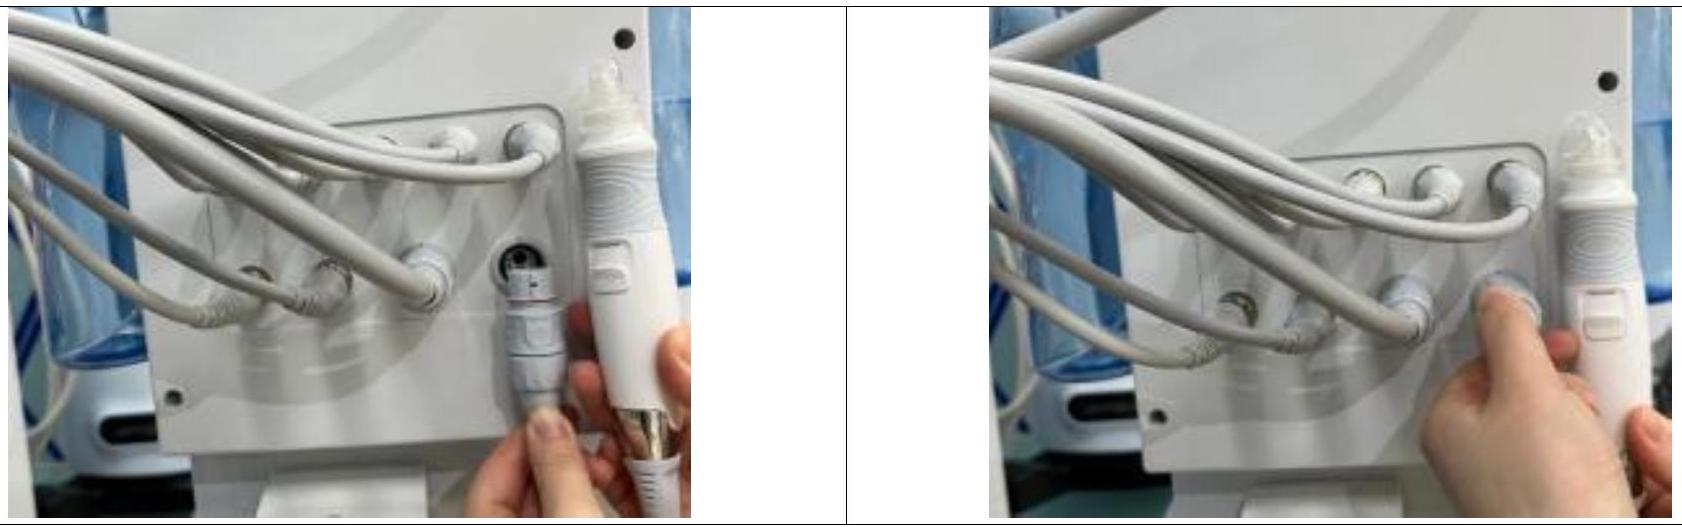
\includegraphics[max width=\textwidth, alt={}, center]{62504995-9f9b-47e6-9021-a213c68ce0b6-19_527_1682_191_187}

\subsection{Installare il filtro}
\begin{center}
\begin{tabular}{|l|l|l|}
\hline
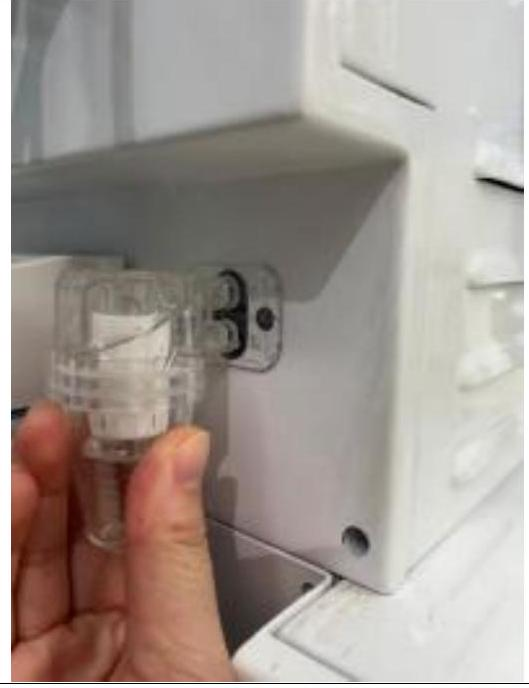
\includegraphics[max width=\textwidth, alt={}]{62504995-9f9b-47e6-9021-a213c68ce0b6-19_688_529_854_225}
 & 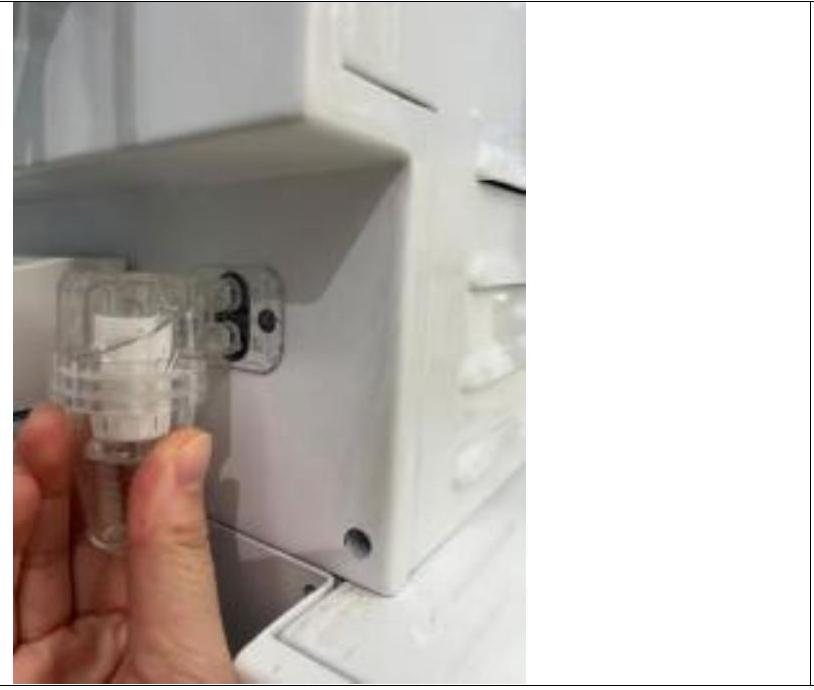
\includegraphics[max width=\textwidth, alt={}]{62504995-9f9b-47e6-9021-a213c68ce0b6-19_690_814_852_223}
 & □ \\
\hline
 &  &  \\
\hline
\end{tabular}
\end{center}

Collegare i filtri come mostrato nell'immagine.

\subsection{Installare il cavo di alimentazione}
\begin{center}
\begin{tabular}{|l|l|}
\hline
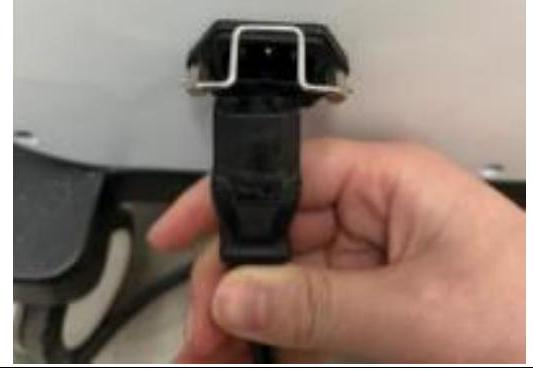
\includegraphics[max width=\textwidth, alt={}]{62504995-9f9b-47e6-9021-a213c68ce0b6-19_370_533_2104_244}
 & 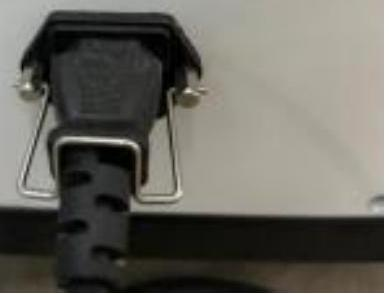
\includegraphics[max width=\textwidth, alt={}]{62504995-9f9b-47e6-9021-a213c68ce0b6-19_294_389_2175_1368}
 \\
\hline
\end{tabular}
\end{center}

\footnotetext{Collegare il cavo di alimentazione e fissarlo come mostrato nell'immagine.
}\section{AVVERTIMENTO:}
\begin{itemize}
  \item Durante il funzionamento, il contenitore di scarico deve essere rimosso e smaltito quando l'acqua di scarico raggiunge i tre quarti bottiglie.\\
-II filtro deve essere premuto con decisione.\\
Dopo aver completato i passaggi di installazione sopra indicati, è possibile utilizzare il cavo di alimentazione per collegarlo al connettore di alimentazione sul retro dello strumento, accenderlo e testarne le prestazioni, dopodiché è possibile utilizzarlo normalmente.
\end{itemize}

\section{Procedura operativa}
\subsection{Requisiti dell'operatore}
\begin{itemize}
  \item L'operatore deve comprendere le conoscenze professionali richieste per utilizzare lo strumento, ricevere una formazione per conformarsi alle leggi locali e nazionali e seguire le migliori pratiche del paese/ regione in cui viene utilizzata la macchina.
  \item Il nucleo della formazione completa della conoscenza.
  \item Avere un'assicurazione completa che copra la responsabilità civile, i rischi relativi al contenuto e al trattamento.\\
4.2 Funzionamento dell'interfaccia
\end{itemize}

Dopo aver acceso la macchina, verranno visualizzate le seguenti interfacce operative (Fig. 1) e (Fig. 2).

\begin{figure}[H]
\begin{center}
  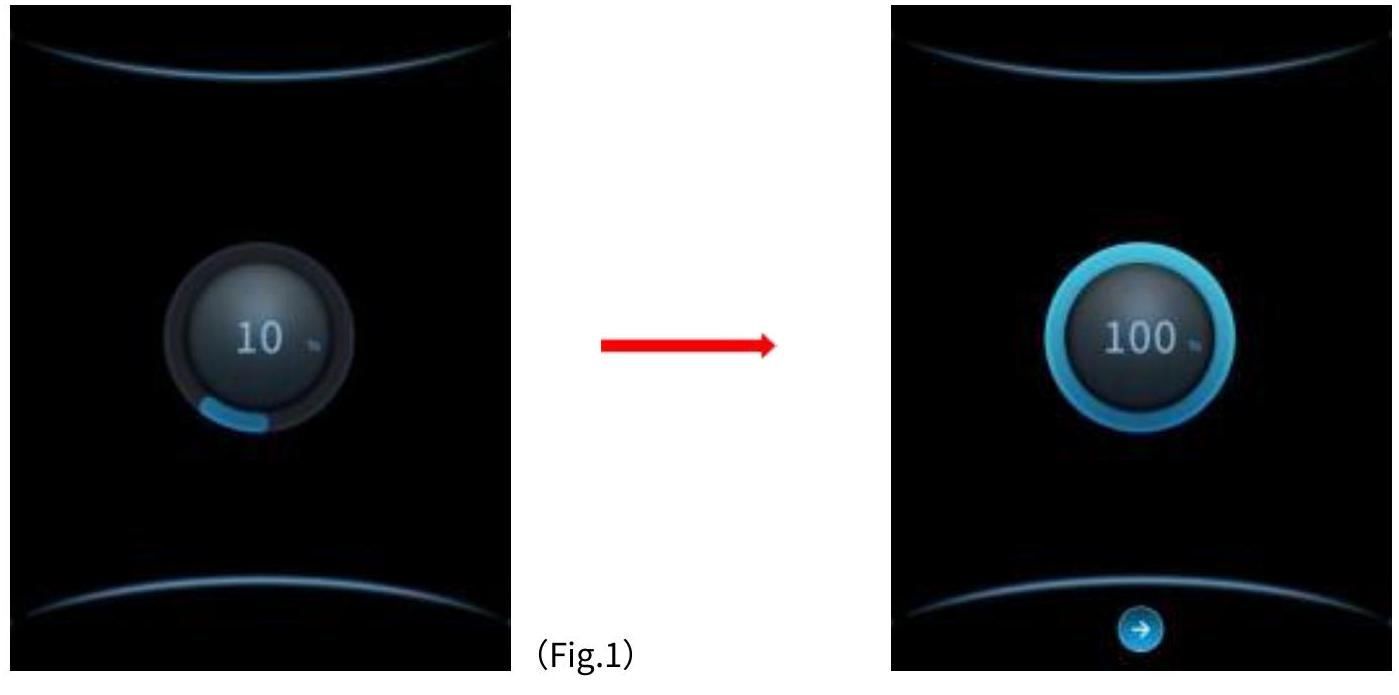
\includegraphics[alt={},max width=\textwidth]{62504995-9f9b-47e6-9021-a213c68ce0b6-21_695_1399_916_221}
\captionsetup{labelformat=empty}
\caption{(Fig.2)}
\end{center}
\end{figure}

quindi fare clic verrà visualizzata la seguente interfaccia operativa (Fig.3).

\begin{figure}[H]
\begin{center}
  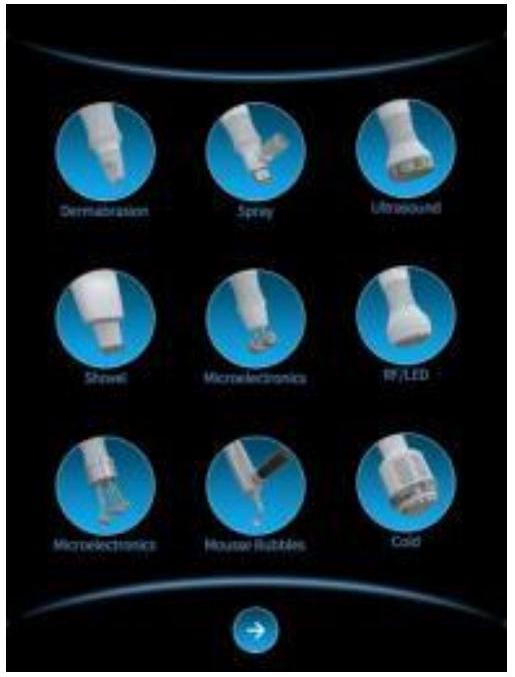
\includegraphics[alt={},max width=\textwidth]{62504995-9f9b-47e6-9021-a213c68ce0b6-21_677_515_1795_680}
\captionsetup{labelformat=empty}
\caption{(Fig.3)}
\end{center}
\end{figure}

Manico per idrodermoabrasione

Clic\\

\includegraphics[max width=\textwidth, alt={}, center]{62504995-9f9b-47e6-9021-a213c68ce0b6-22_250_243_255_315}\\
e poi premere

\begin{figure}[H]
\begin{center}
  
\includegraphics[alt={},max width=\textwidth]{62504995-9f9b-47e6-9021-a213c68ce0b6-22_127_145_383_817}
\captionsetup{labelformat=empty}
\caption{per accedere all'interfaccia successiva (Fig. 4).}
\end{center}
\end{figure}

\begin{center}
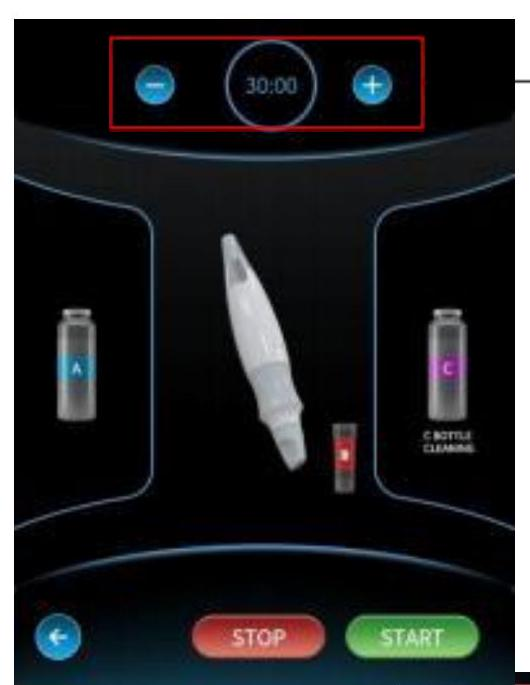
\includegraphics[max width=\textwidth, alt={}]{62504995-9f9b-47e6-9021-a213c68ce0b6-22_685_530_548_709}
\end{center}

Tempo di trattamento

Clic\\
la macchina può iniziare a funzionare. Fare clic\\
la macchina smette di funzionare. Dopo l'uso\\
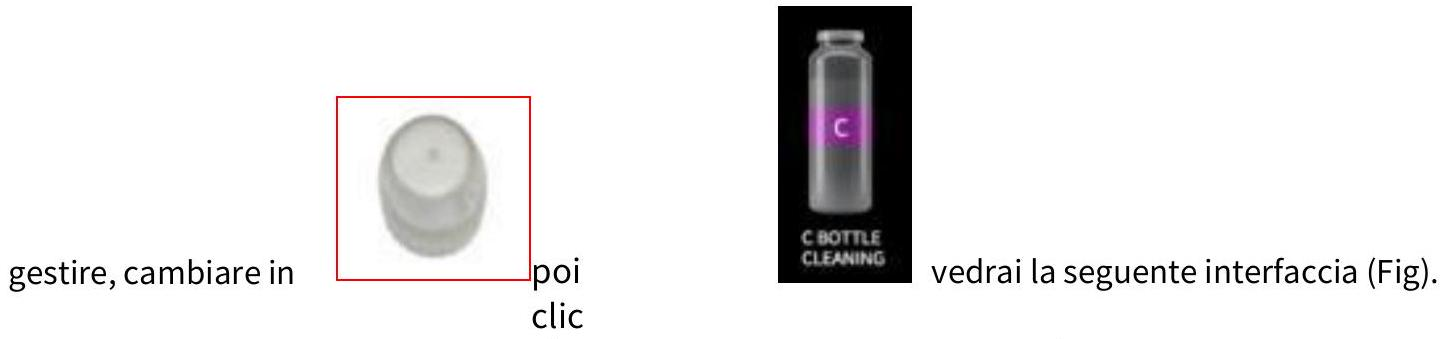
\includegraphics[max width=\textwidth, alt={}, center]{62504995-9f9b-47e6-9021-a213c68ce0b6-22_339_1451_1334_169}

\begin{figure}[H]
\begin{center}
  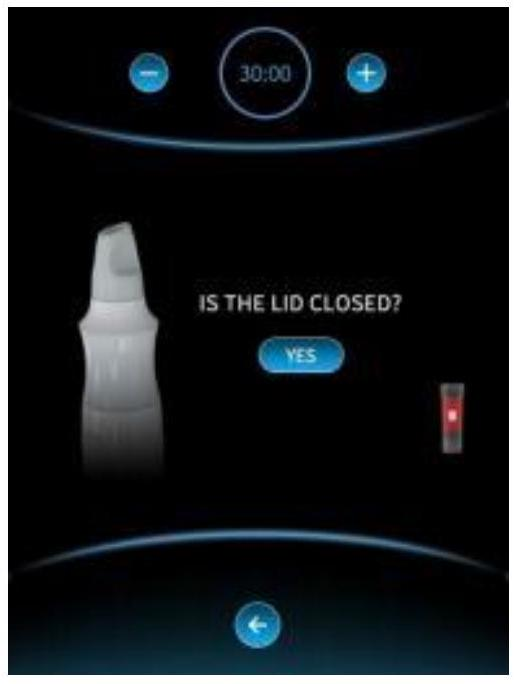
\includegraphics[alt={},max width=\textwidth]{62504995-9f9b-47e6-9021-a213c68ce0b6-22_684_517_1672_719}
\captionsetup{labelformat=empty}
\caption{(Figura 5)}
\end{center}
\end{figure}

Quindi fare clic\\
la macchina si pulirà automaticamente.

\section{Manico in schiuma a bolle}
\begin{center}
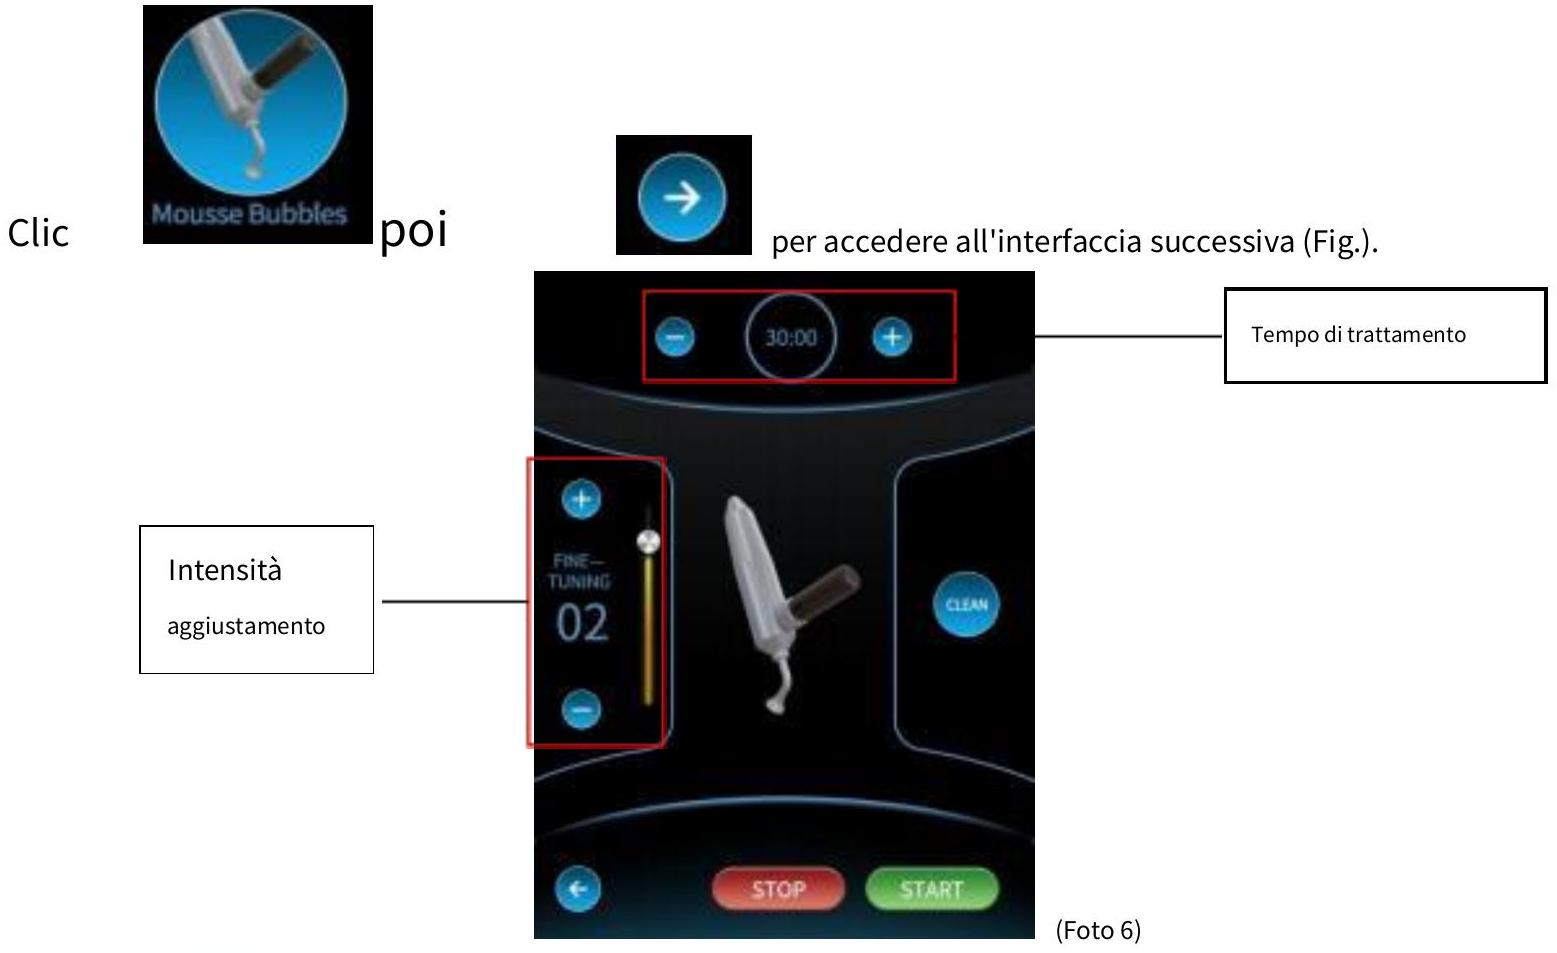
\includegraphics[max width=\textwidth, alt={}]{62504995-9f9b-47e6-9021-a213c68ce0b6-23_953_1557_251_189}
\end{center}

\section{START}
Clic\\
la macchina può iniziare a lavorare. Fare clic\\
la maniglia, iniettare acqua calda a circa $40^{\circ} \mathrm{C}$ in un'altra bottiglia e quindi fare clic per pulire la maniglia.

\section{Impugnatura spray atomizzatrice polimerica}
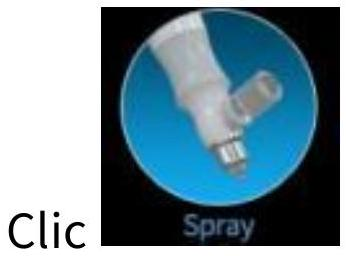
\includegraphics[max width=\textwidth, alt={}, center]{62504995-9f9b-47e6-9021-a213c68ce0b6-23_256_346_1631_191}\\
e poi premere\\

\includegraphics[max width=\textwidth, alt={}, center]{62504995-9f9b-47e6-9021-a213c68ce0b6-23_131_154_1763_822}\\
per accedere all'interfaccia successiva (Fig.7).\\
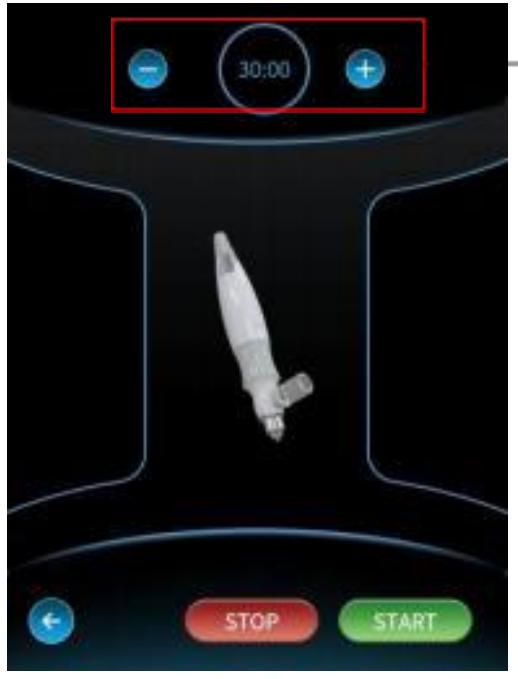
\includegraphics[max width=\textwidth, alt={}, center]{62504995-9f9b-47e6-9021-a213c68ce0b6-23_679_518_1896_680}\\
(Foto 7)

\section{Maniglia a vibrazione ultrasonica}
\section{Clic Shovel e poi premere per accedere all'interfaccia successiva (Fig.8).}
\begin{center}
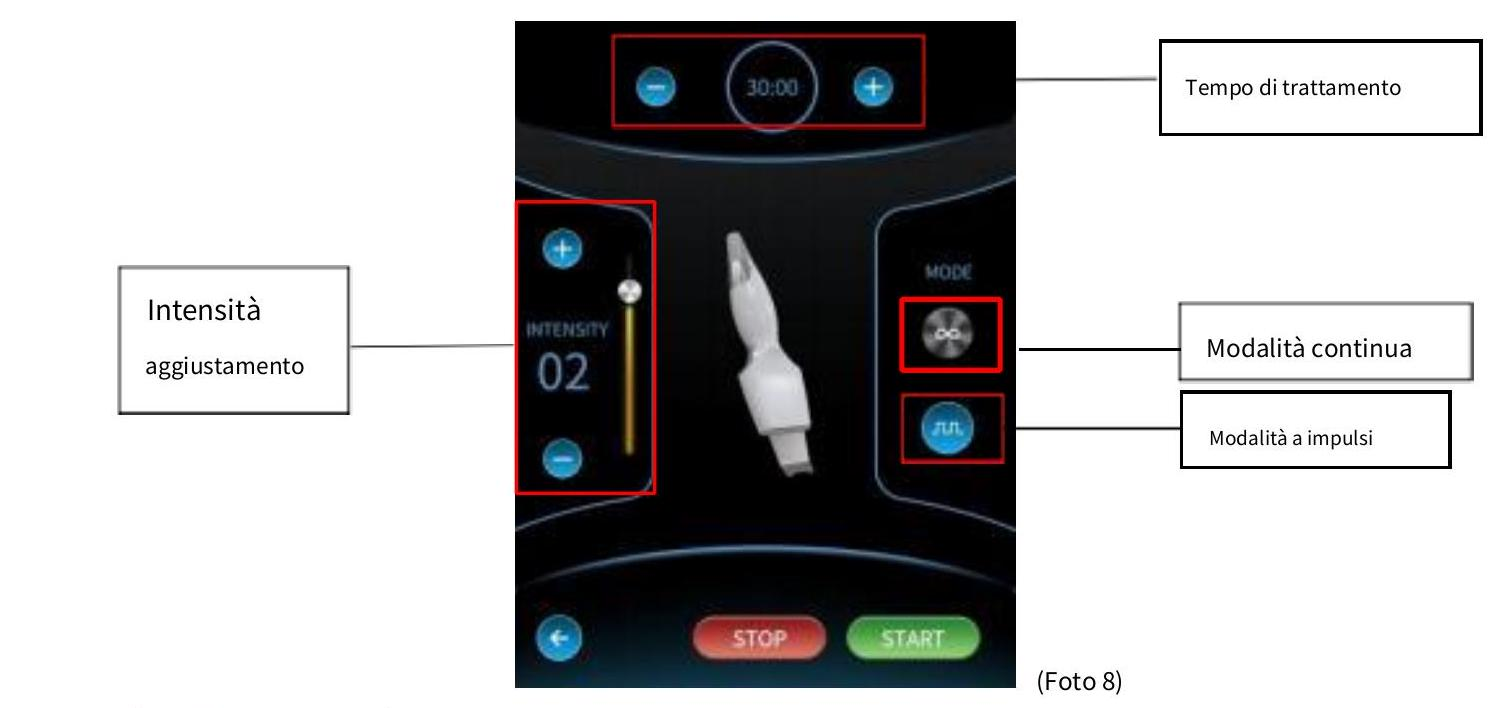
\includegraphics[max width=\textwidth, alt={}]{62504995-9f9b-47e6-9021-a213c68ce0b6-24_708_1492_701_153}
\end{center}

\begin{figure}[H]
\begin{center}
  
\includegraphics[alt={},max width=\textwidth]{62504995-9f9b-47e6-9021-a213c68ce0b6-24_126_277_1407_269}
\captionsetup{labelformat=empty}
\caption{la macchina può iniziare a lavorare. Fare clic}
\end{center}
\end{figure}


\includegraphics[max width=\textwidth, alt={}, center]{62504995-9f9b-47e6-9021-a213c68ce0b6-24_108_268_1425_1110}\\
la macchina smetterà di funzionare.

\section{Maniglia RF bipolare}
Clic\\
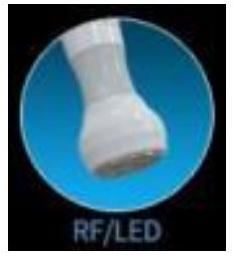
\includegraphics[max width=\textwidth, alt={}, center]{62504995-9f9b-47e6-9021-a213c68ce0b6-24_257_237_1667_287}\\
e poi premere\\

\includegraphics[max width=\textwidth, alt={}, center]{62504995-9f9b-47e6-9021-a213c68ce0b6-24_134_150_1795_799}\\
per accedere all'interfaccia successiva (Fig.9).\\
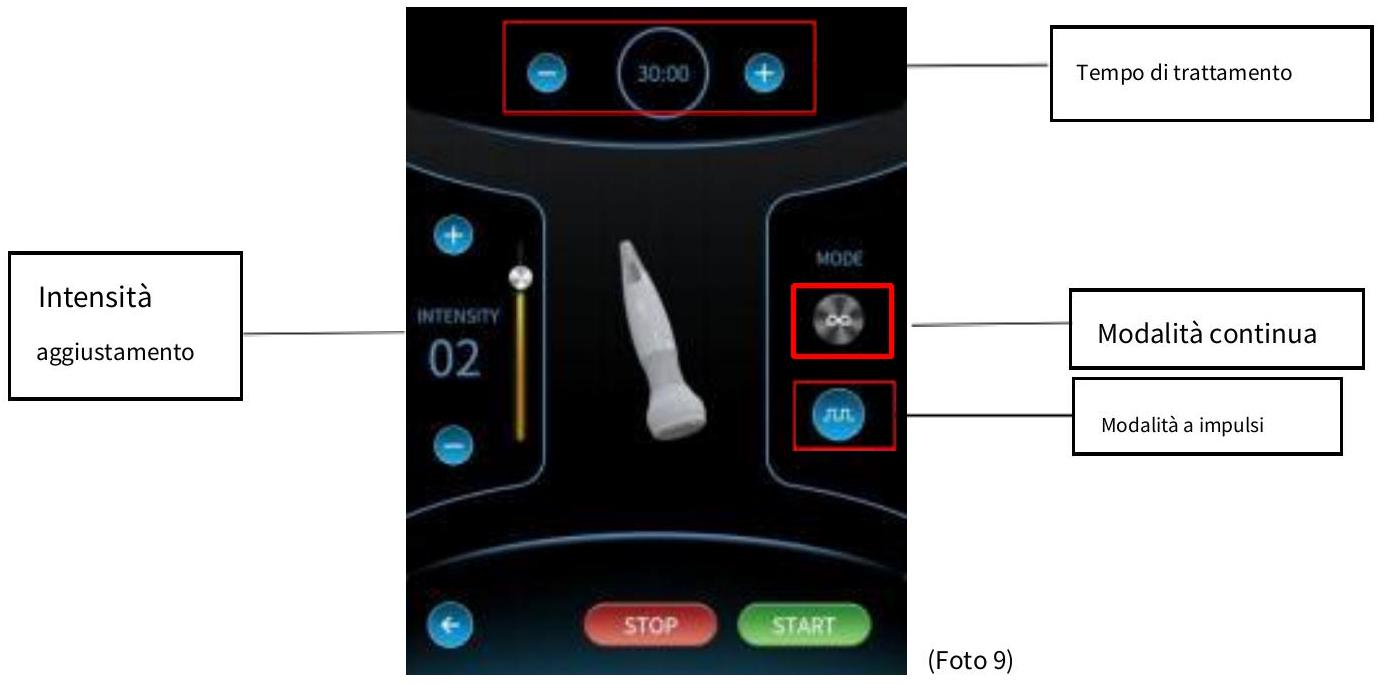
\includegraphics[max width=\textwidth, alt={}, center]{62504995-9f9b-47e6-9021-a213c68ce0b6-24_684_1381_1941_262}\\
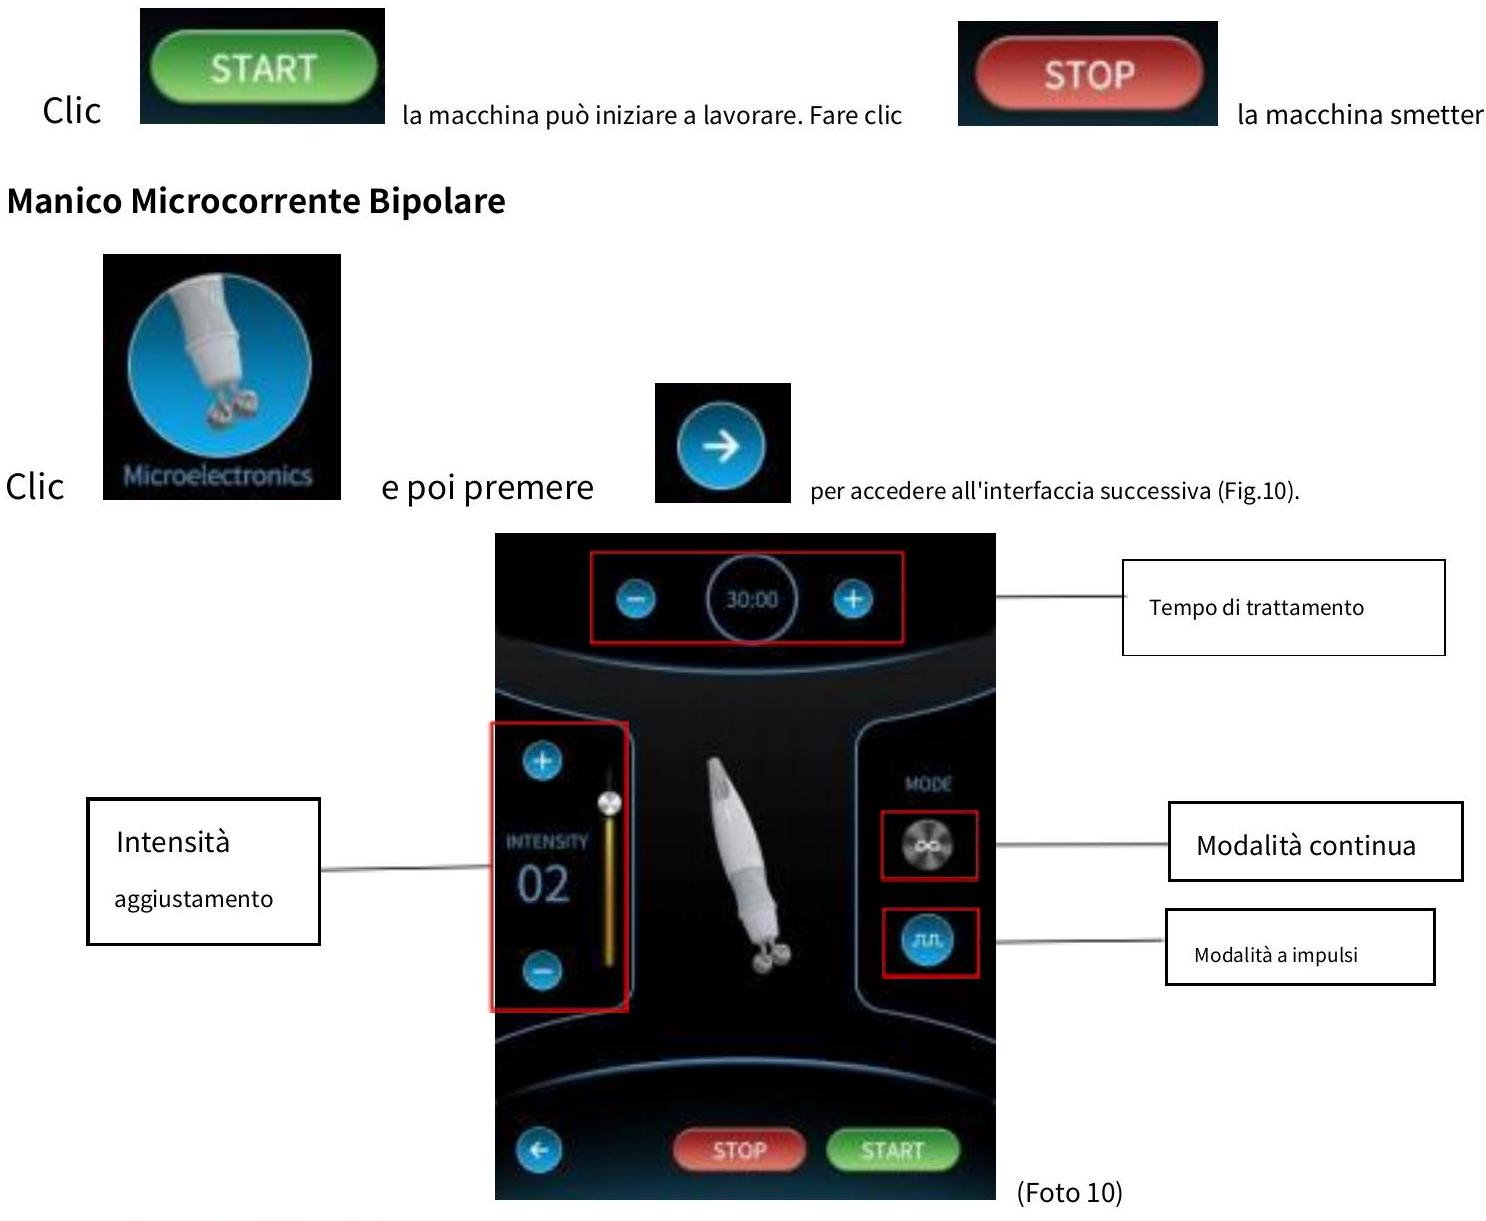
\includegraphics[max width=\textwidth, alt={}, center]{62504995-9f9b-47e6-9021-a213c68ce0b6-25_1221_1486_189_155}

Clic

\begin{figure}[H]
\begin{center}
  
\includegraphics[alt={},max width=\textwidth]{62504995-9f9b-47e6-9021-a213c68ce0b6-25_122_277_1411_269}
\captionsetup{labelformat=empty}
\caption{la macchina può iniziare a lavorare. Fare clic}
\end{center}
\end{figure}


\includegraphics[max width=\textwidth, alt={}, center]{62504995-9f9b-47e6-9021-a213c68ce0b6-25_113_268_1425_1110}\\
la macchina smetterà di funzionare.

\section{Manipolo microcorrente multipolare}
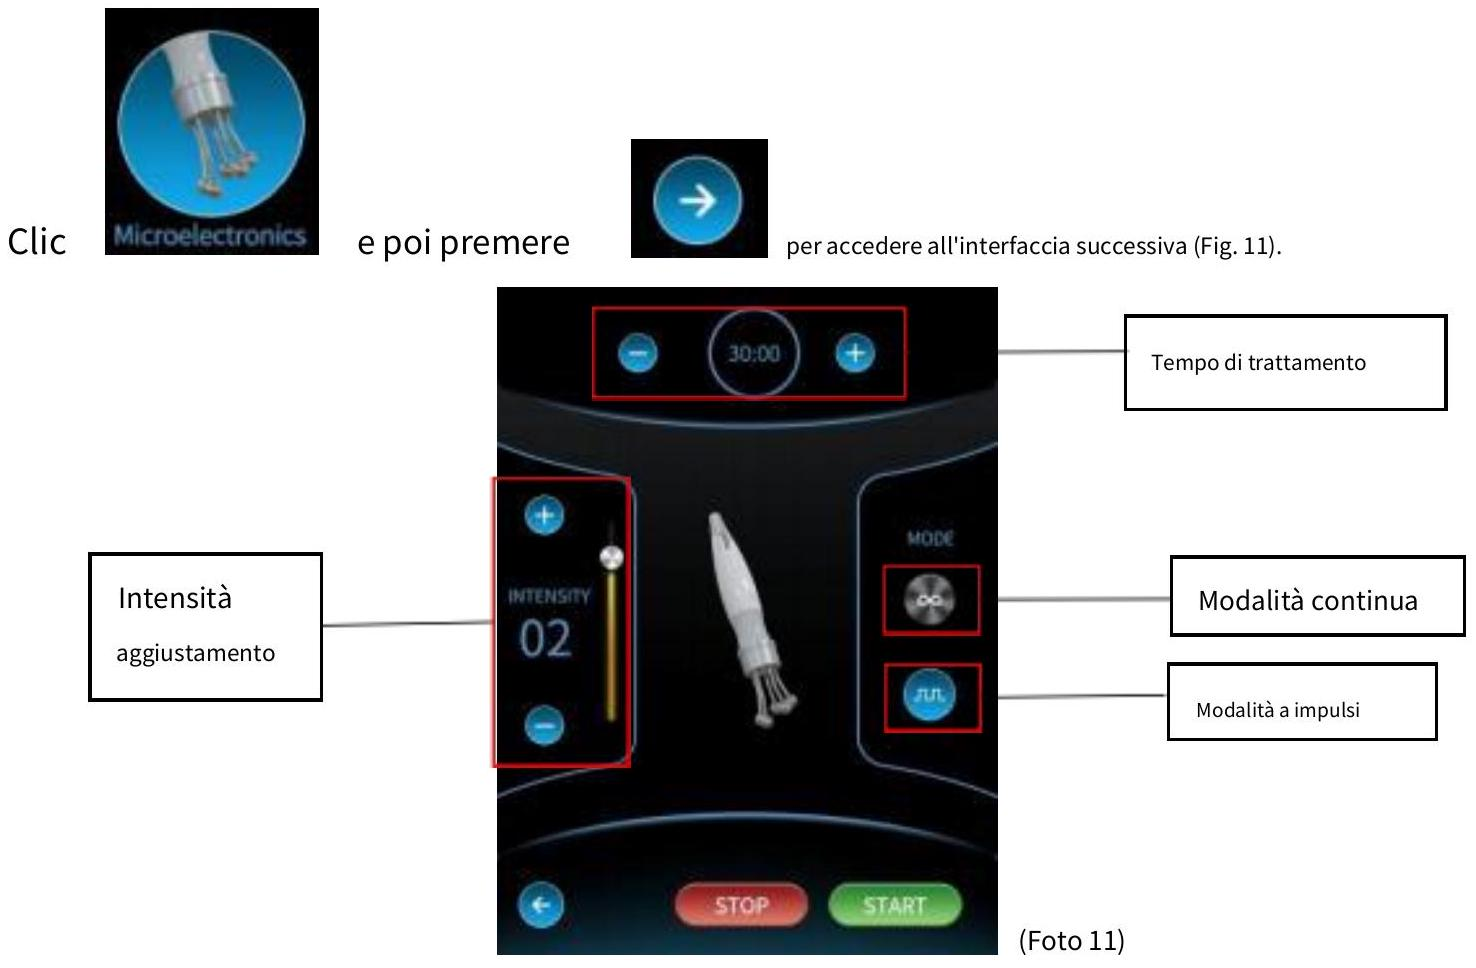
\includegraphics[max width=\textwidth, alt={}, center]{62504995-9f9b-47e6-9021-a213c68ce0b6-25_968_1476_1653_153}\\
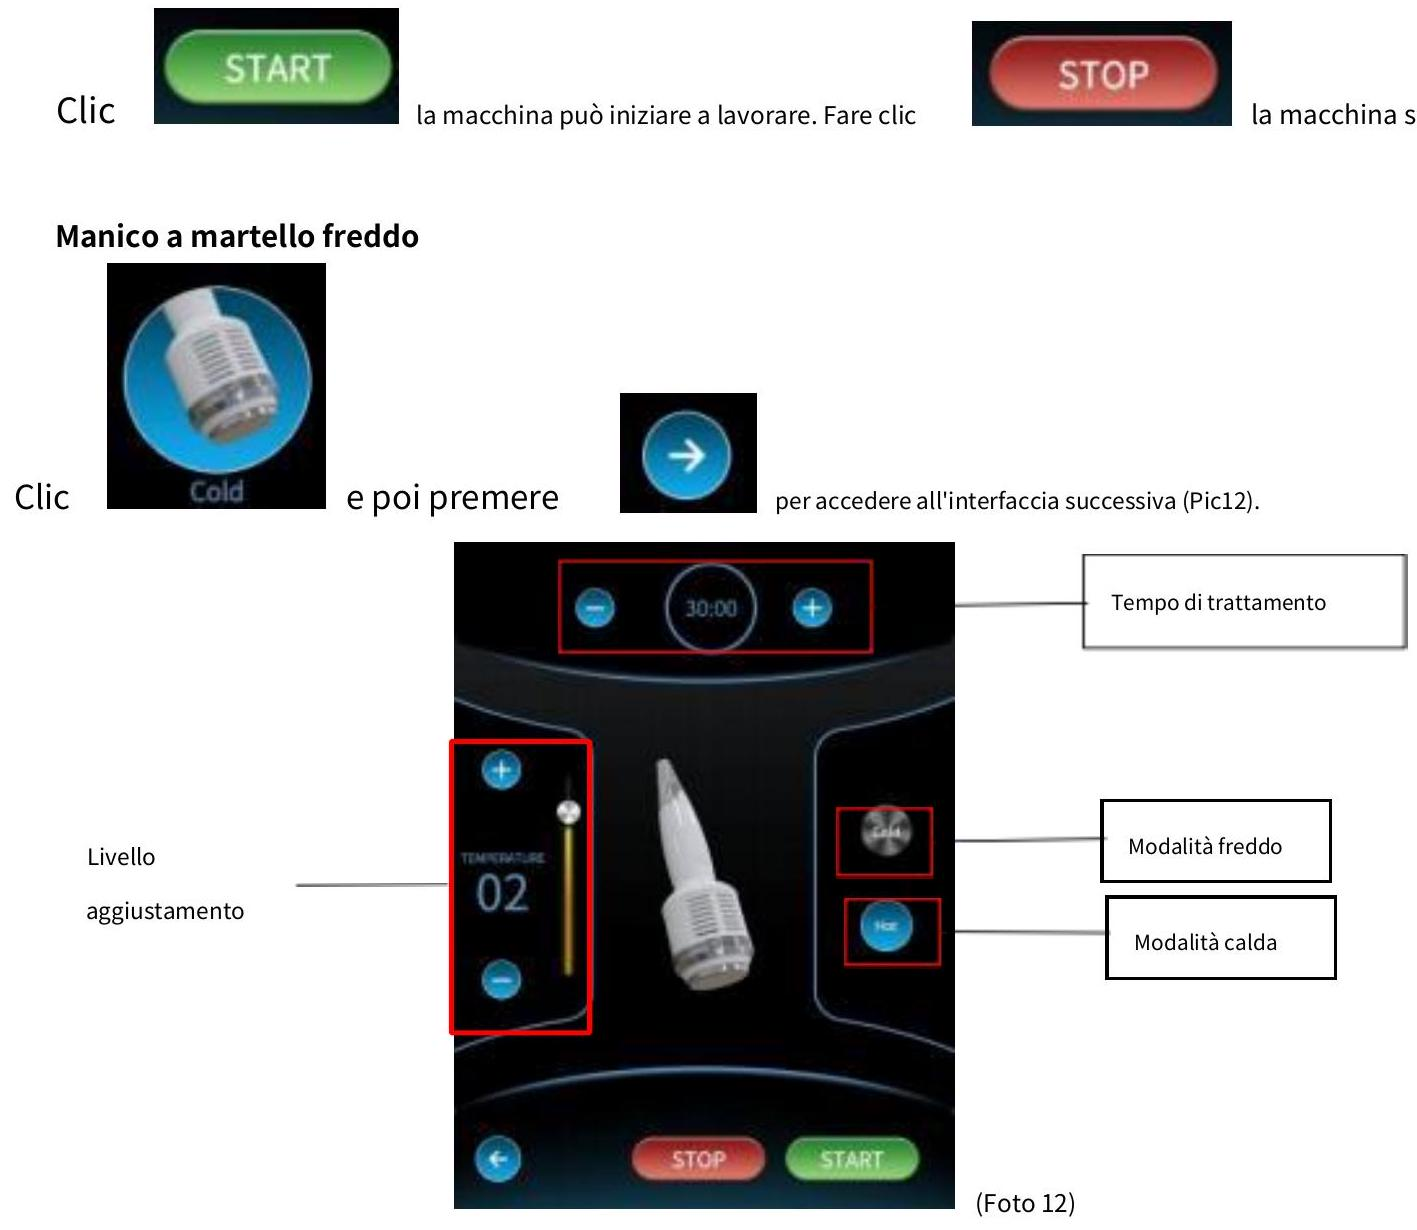
\includegraphics[max width=\textwidth, alt={}, center]{62504995-9f9b-47e6-9021-a213c68ce0b6-26_1230_1417_189_141}

\section{Handle di importazione degli ultrasuoni}
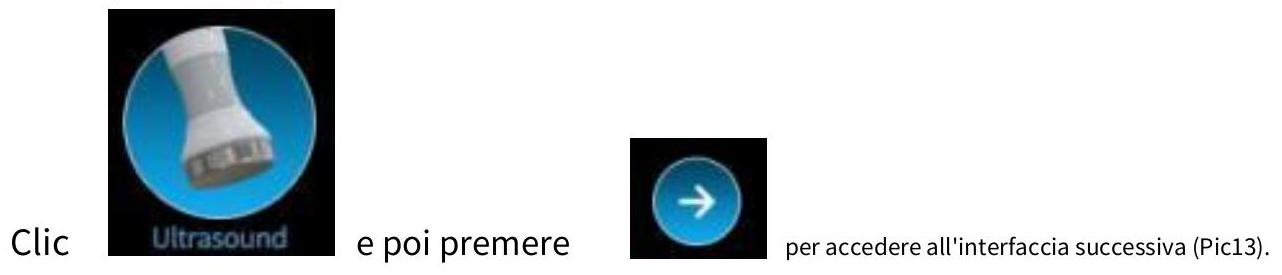
\includegraphics[max width=\textwidth, alt={}, center]{62504995-9f9b-47e6-9021-a213c68ce0b6-26_275_1282_1852_187}\\
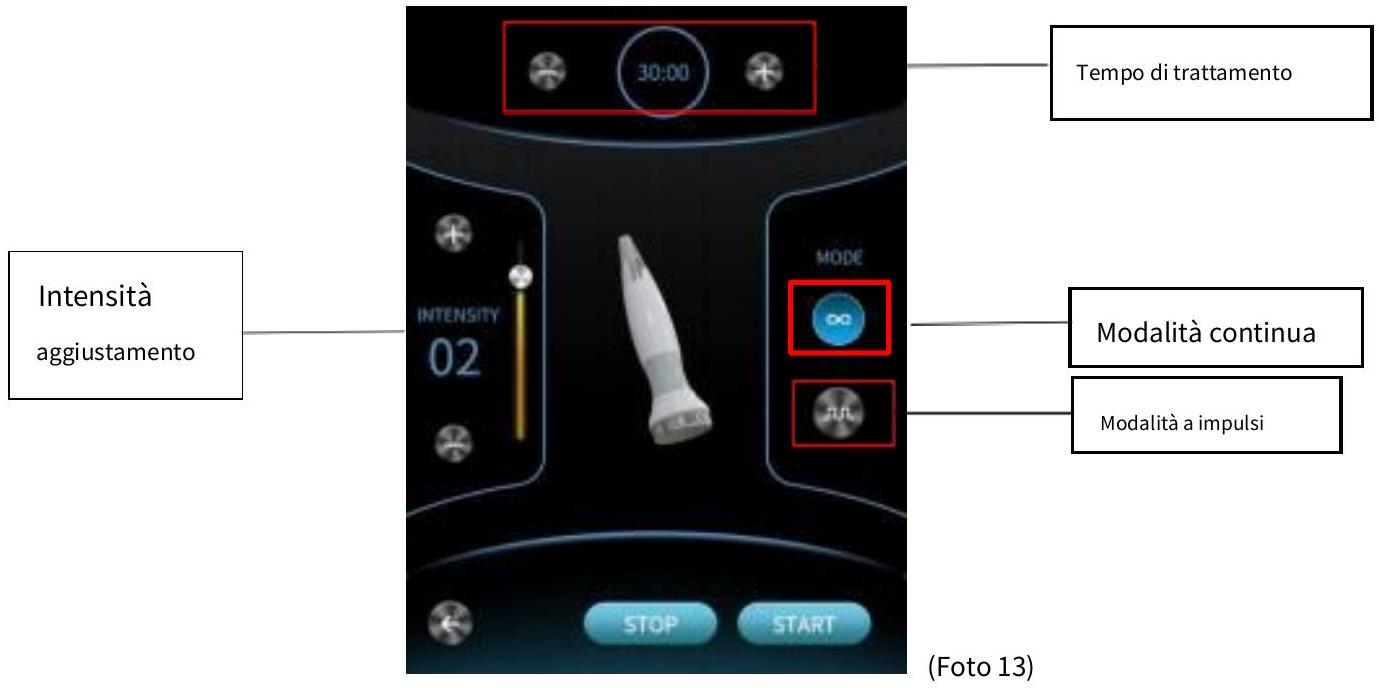
\includegraphics[max width=\textwidth, alt={}, center]{62504995-9f9b-47e6-9021-a213c68ce0b6-27_688_1379_201_262}

\section{Il funzionamento della macchina}
\subsection{Consulenza al cliente}
Prima di qualsiasi trattamento è necessario effettuare una consulenza approfondita e un test cutaneo.\\
Effettua una consulenza privata per far sentire i clienti a proprio agio. La consulenza ti permetterà di valutare se il cliente è idoneo al trattamento.

Durante la consulenza, è necessario trattare i seguenti punti e creare un profilo del cliente da aggiornare nei futuri appuntamenti:

\begin{enumerate}
  \item Tabella completa dei tipi di pelle
\end{enumerate}

2 Ottenere informazioni personali sui clienti\\
3. Completare la cartella clinica per determinare se il cliente è idoneo al trattamento\\
4. Spiegare come funziona il processo operativo\\
5. Cure post-trattamento\\
6. Raccomandazioni pre-trattamento per appuntamenti futuri\\
7. Storia del trattamento

\subsection{Trattamento delle maniglie}
\subsubsection{Manico a bolle di mousse}
Fare clic sull'icona della maniglia delle bolle di mousse e impostare l'intensità da 3 . Una volta che le bolle si sono normalizzate, ridurre l'intensità a 1. Utilizzare 3 asciugamani per coprire occhi e bocca. Quindi, far coprire il viso con le bolle per 1-2 minuti (il corpo per 2-3 minuti) con un\\
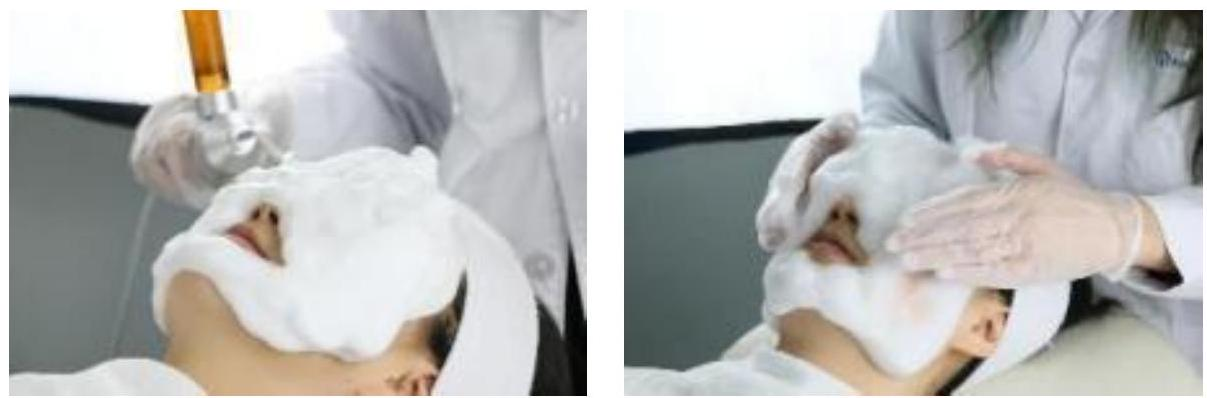
\includegraphics[max width=\textwidth, alt={}, center]{62504995-9f9b-47e6-9021-a213c68ce0b6-28_398_1207_1537_815}\\
massaggio appropriato. Al termine del trattamento, asciugare le bolle con l'asciugamano e acqua salina.

Dopo ogni trattamento,noi dovere pulito IL maniglia E sostituzione due pezzi Di cotone fogli altro Di corlL\\
maniglia È intasato.

\begin{figure}[H]
\begin{center}
  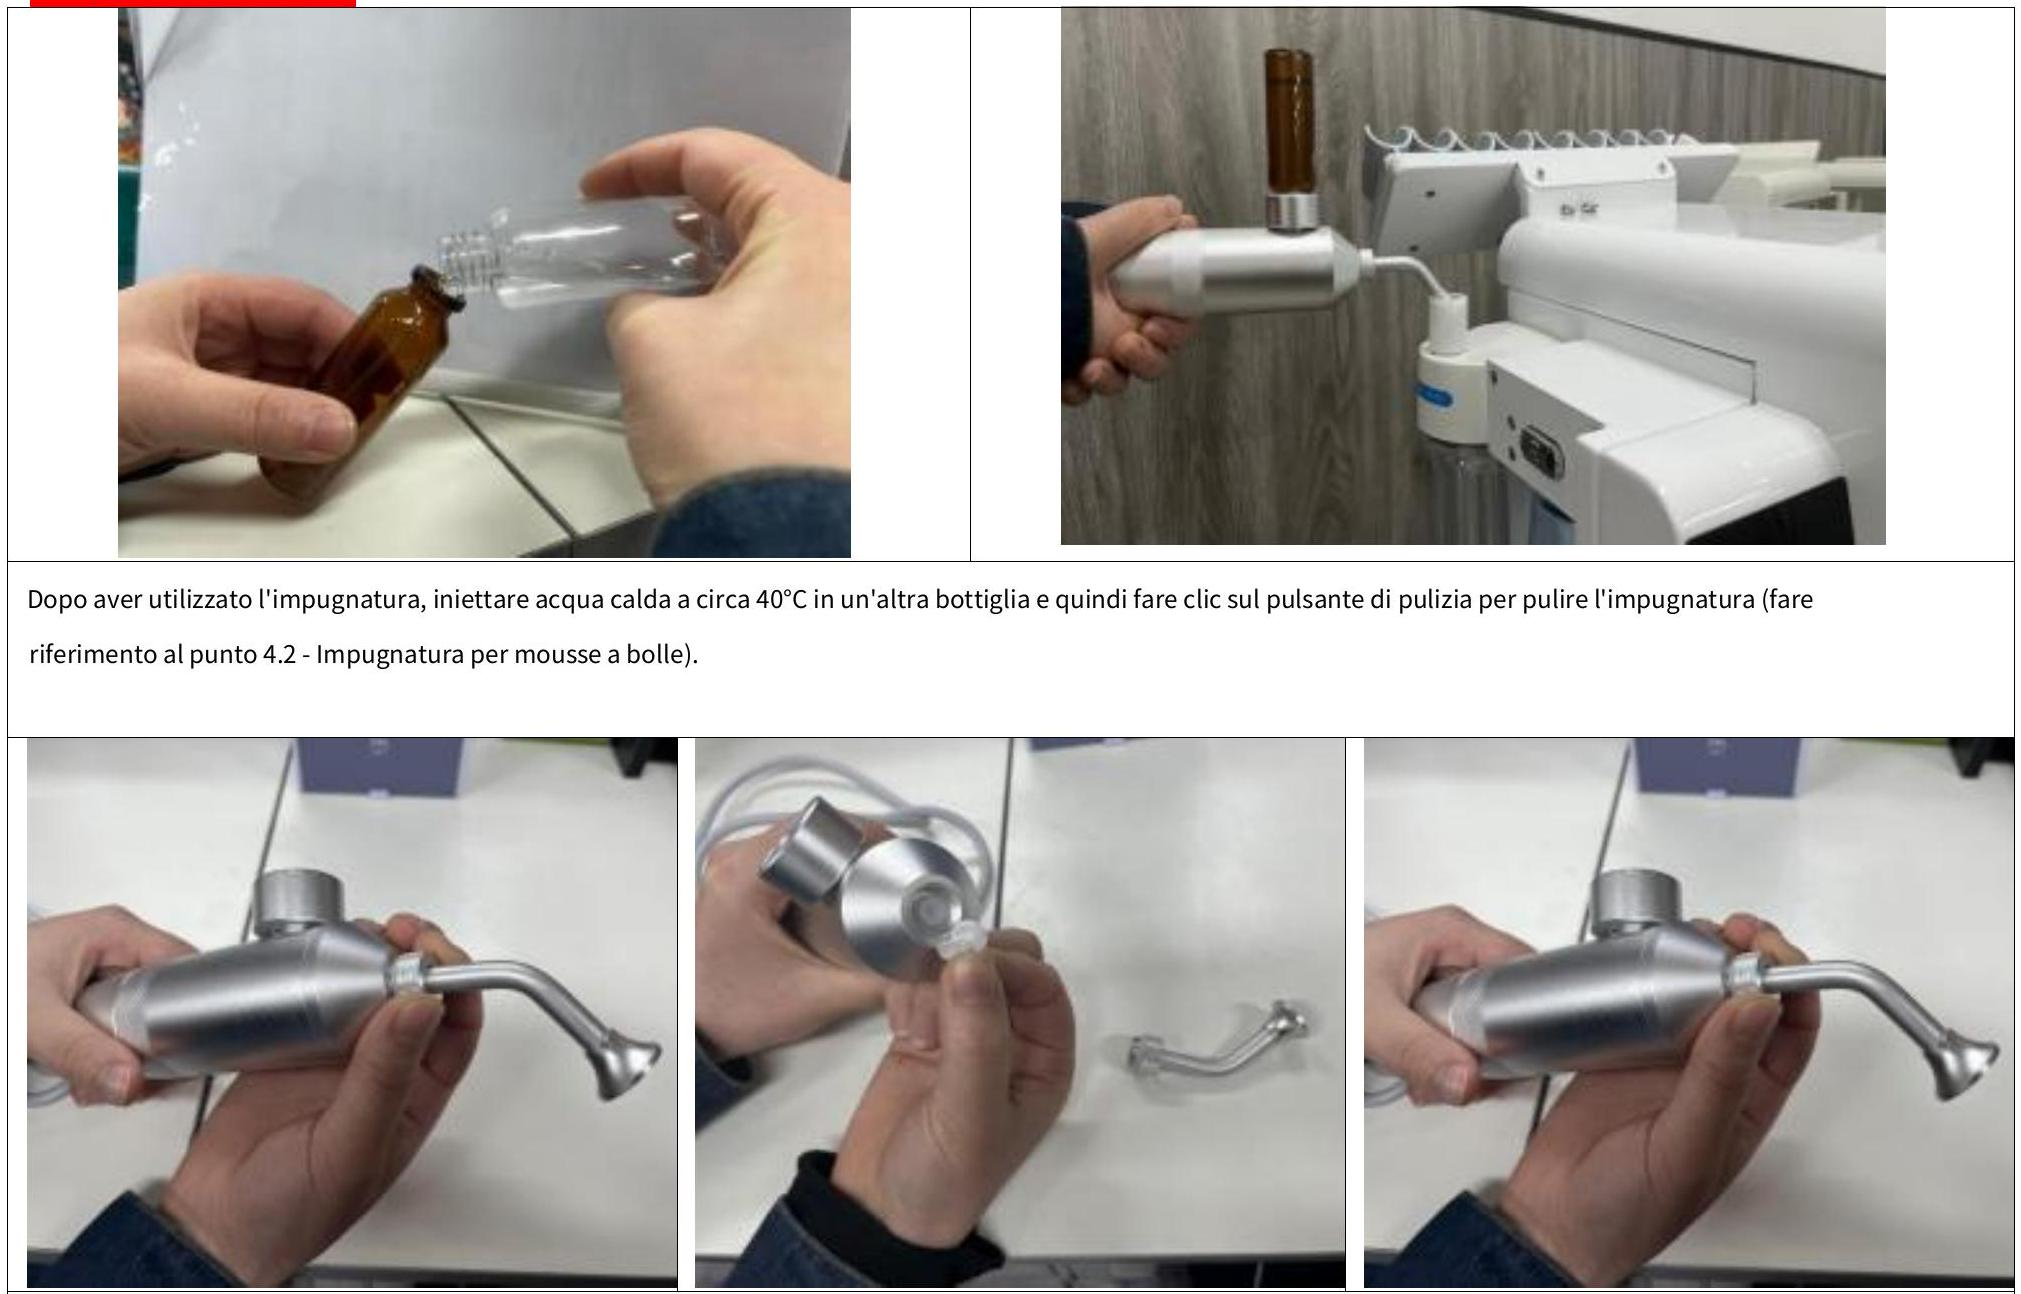
\includegraphics[alt={},max width=\textwidth]{62504995-9f9b-47e6-9021-a213c68ce0b6-29_1294_2021_310_22}
\captionsetup{labelformat=empty}
\caption{Svitare la parte metallica dell'impugnatura, sostituire i due pezzi di lenzuola di cotone (vedere 3.1-14). Quindi avvitare la parte mentale.}
\end{center}
\end{figure}

\begin{center}
\begin{tabular}{l|l|l|l|l|l|l|}
\hline
Se le bolle non sono dense & O IL La maniglia è intasata. & , modifica & IL pipe Di IL mousse & bolla \\
maniglia (fare riferimento a 3.1-15) e il filtro( arbitro a 3.1-7).Come mostrato di seguito . &  &  &  &  \\
\end{tabular}
\end{center}

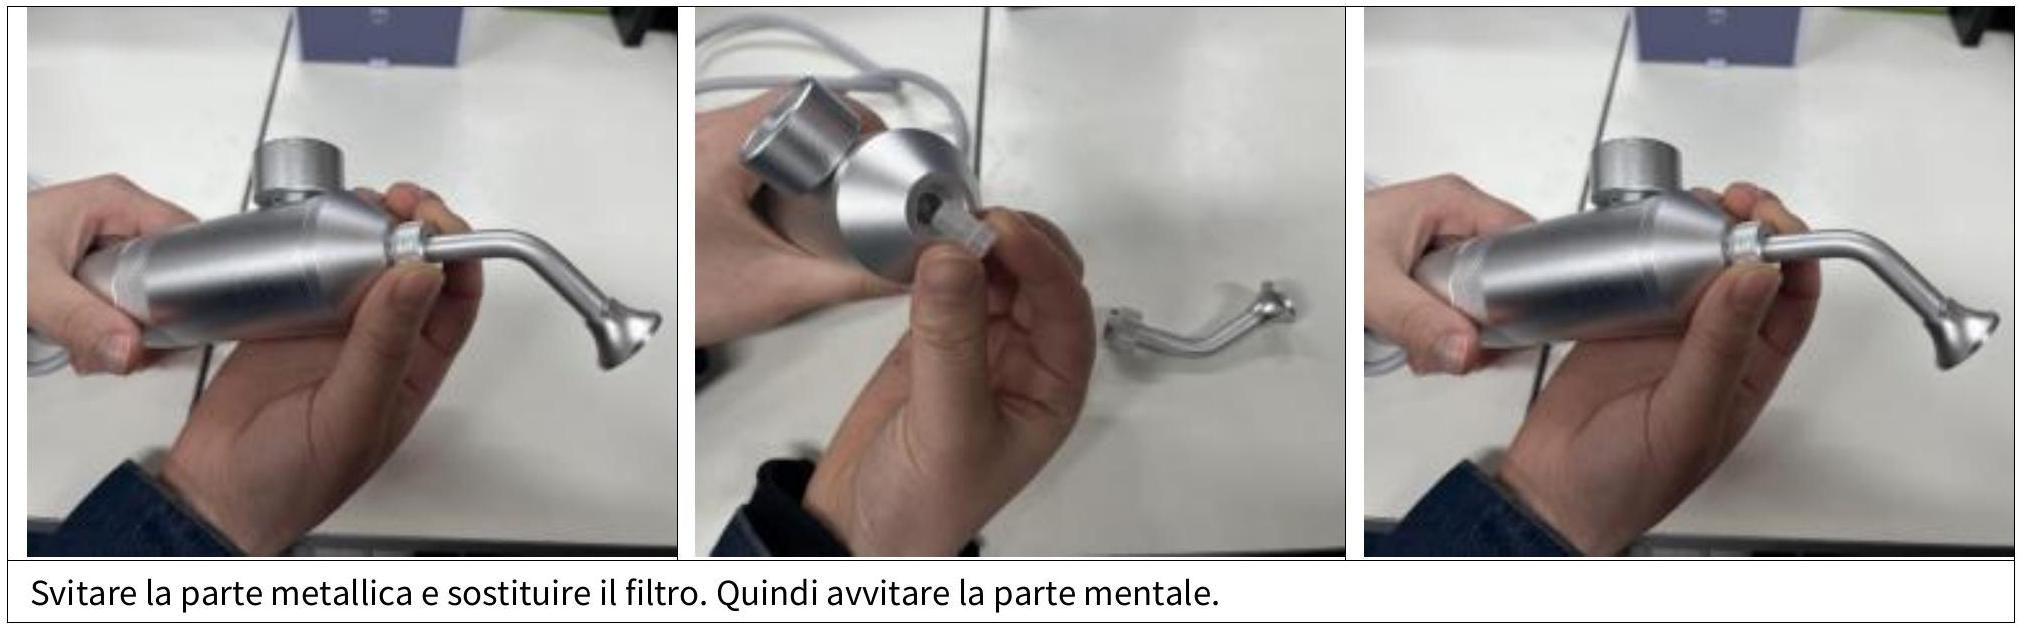
\includegraphics[max width=\textwidth, alt={}, center]{62504995-9f9b-47e6-9021-a213c68ce0b6-29_630_2021_1959_22}\\
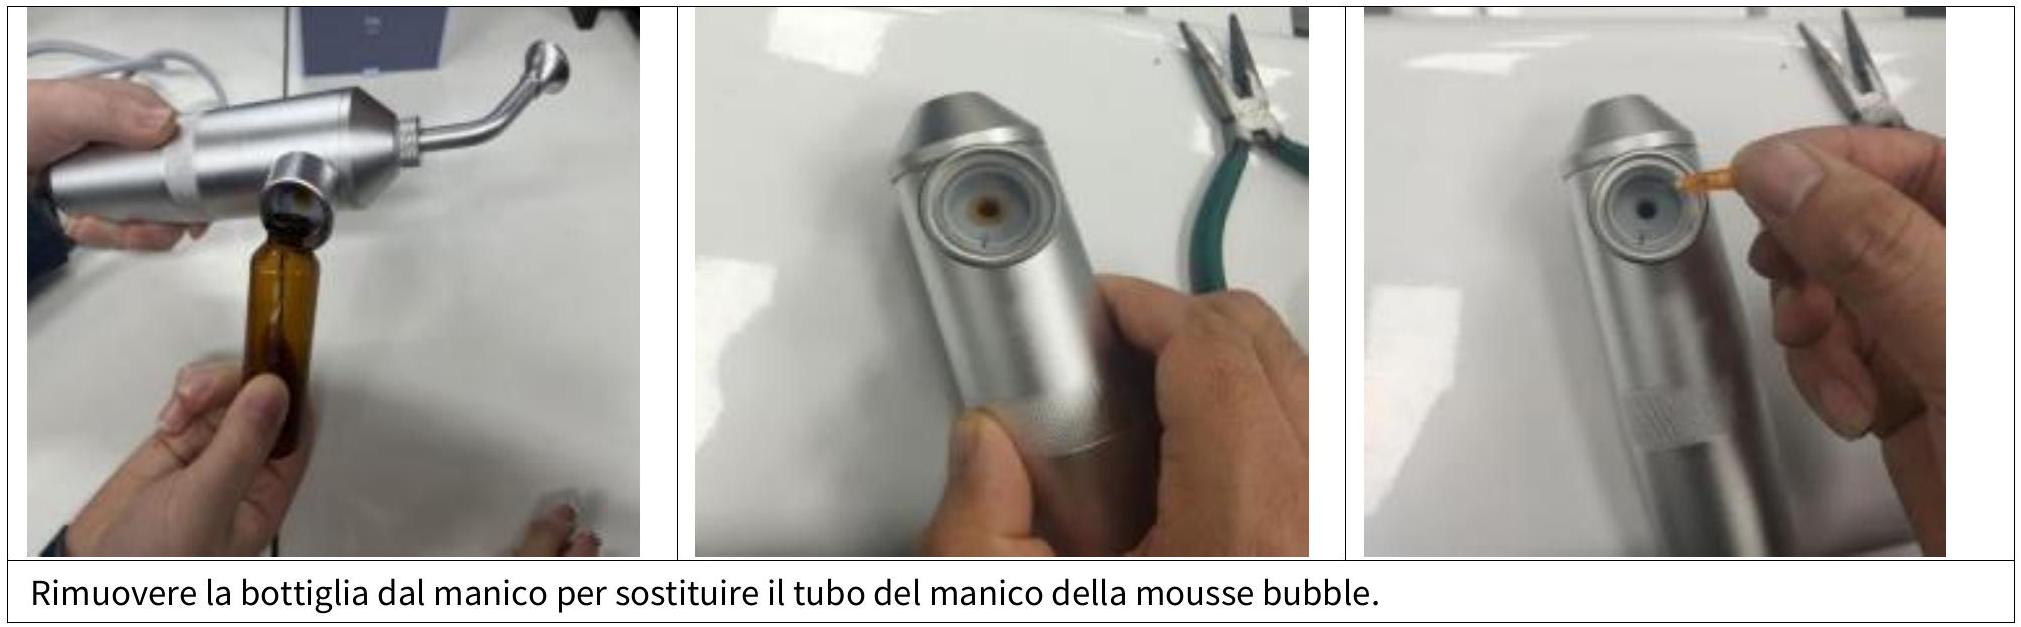
\includegraphics[max width=\textwidth, alt={}, center]{62504995-9f9b-47e6-9021-a213c68ce0b6-30_627_2021_191_22}

\subsubsection{Manico per idrodermoabrasione}
Si consiglia di utilizzare lo spray caldo per 10 minuti aprire i pori, quindi scegliere un tappo adatto di conseguenza la pelle, regolare la giusta potenza di aspirazione, la giusta quantità di acqua.\\
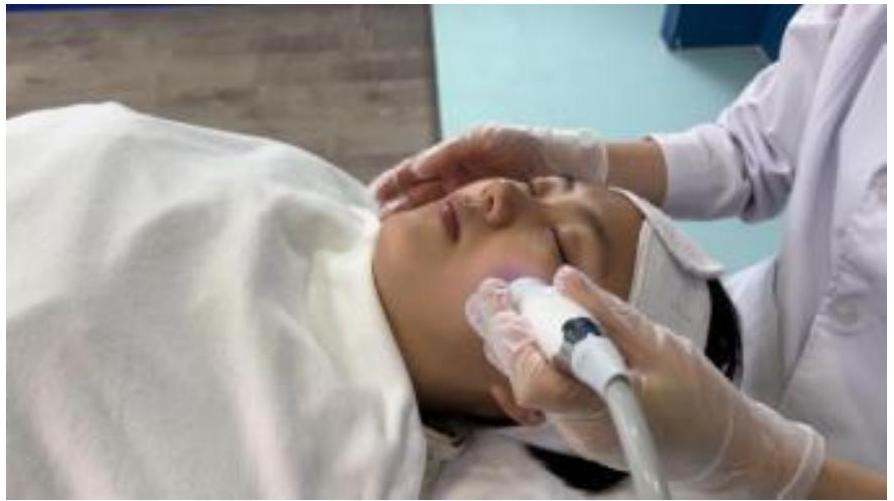
\includegraphics[max width=\textwidth, alt={}, center]{62504995-9f9b-47e6-9021-a213c68ce0b6-30_501_894_959_1069}

\begin{center}
\begin{tabular}{|l|l|l|l|l|}
\hline
\begin{tabular}{l}
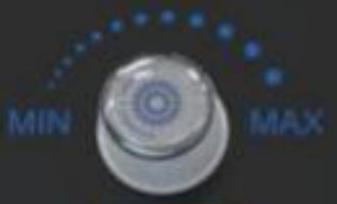
\includegraphics[max width=\textwidth, alt={}]{62504995-9f9b-47e6-9021-a213c68ce0b6-30_204_337_1574_220}
 \\
WATER \\
\end{tabular} &  & \begin{tabular}{l}
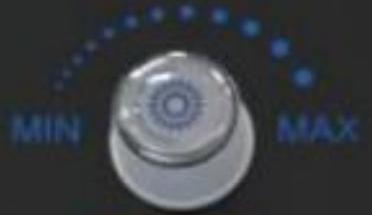
\includegraphics[max width=\textwidth, alt={}]{62504995-9f9b-47e6-9021-a213c68ce0b6-30_215_372_1567_864}
 \\
AIR \\
\end{tabular} &  & 
\includegraphics[max width=\textwidth, alt={}]{62504995-9f9b-47e6-9021-a213c68ce0b6-30_244_301_1564_1524}
 \\
\hline
\multicolumn{2}{|c|}{Ruotare questa manopola per regolare la quantità di acqua in uscita.} & \multicolumn{2}{|c|}{Ruotare questa manopola per regolare l'aspirazione dell'aria.} & Ruotare questa manopola per scegliere la bottiglia. \\
\hline
\end{tabular}
\end{center}

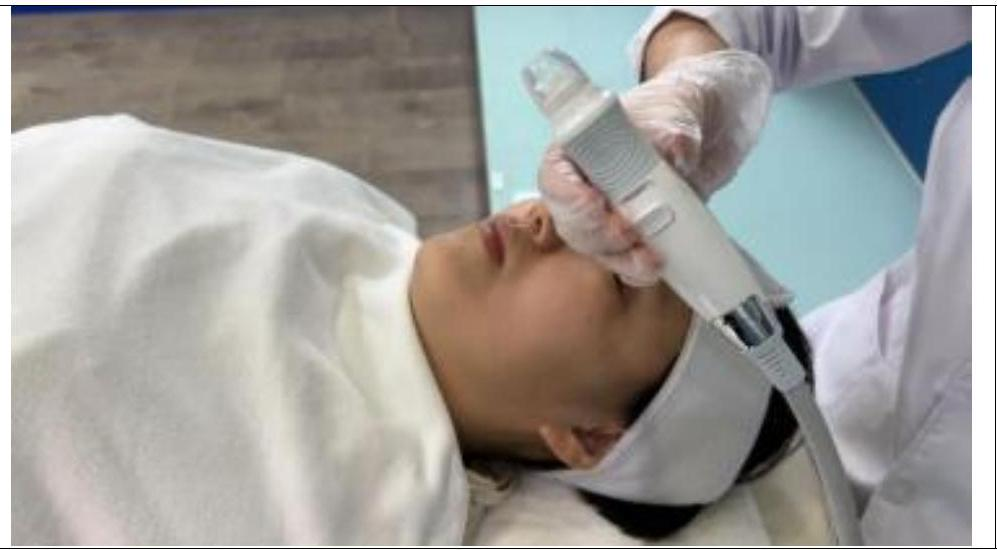
\includegraphics[max width=\textwidth, alt={}, center]{62504995-9f9b-47e6-9021-a213c68ce0b6-31_550_997_312_38}\\
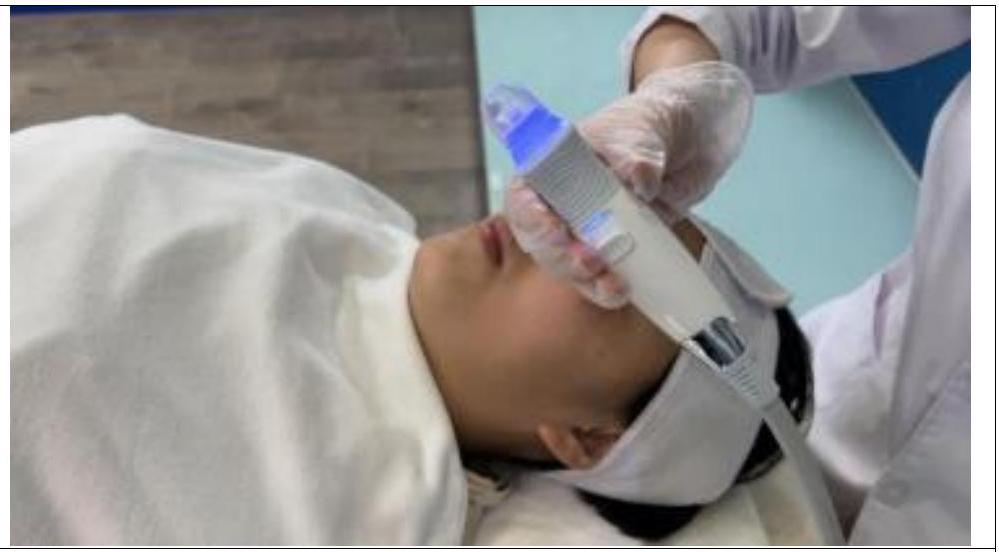
\includegraphics[max width=\textwidth, alt={}, center]{62504995-9f9b-47e6-9021-a213c68ce0b6-31_552_999_312_1041}

Sostituire il cappuccio di pulizia e quindi fare clic su Pulizia; la pulizia avverrà automaticamente per 45 secondi (per i passaggi dettagliati, fare riferimento al punto 4.2 Impugnatura per idrodermoabrasione).

\begin{itemize}
  \item Testina morbida per dermoabrasione ad acqua: adatta a pelli sottili e sensibili
  \item Testina dura per dermoabrasione ad acqua: adatta a pelli normali
  \item Testa dura smerigliata al diamante: adatta per lo strato corneo più spesso (ha l'effetto della dermoabrasione)
  \item La testina per dermoabrasione ad acqua ha tre funzioni, e la testina per dermoabrasione ad acqua per ogni effetto ha dimensioni grandi, medie e piccole. L'operatore sceglie la testina in base all'area della parte. Il funzionamento Il metodo si basa sulla consistenza della pelle dal basso verso l'alto. Ogni linea si percorre per una breve distanza tra le orecchie e l'attaccatura dei capelli (nota: pelle sensibile, allergica, fragile, gravemente acneica, questa funzione non è consigliata).
\end{itemize}

\subsubsection{Impugnatura per nebulizzatore polimerico}
Versare un po' di tonico liquido funzionale nel flacone con il manico e tracciare un cerchio a $2-3 \mathrm{~cm}$ di distanza dal viso. Il trattamento può essere effettuato su tutto il viso per 10-15 minuti.\\
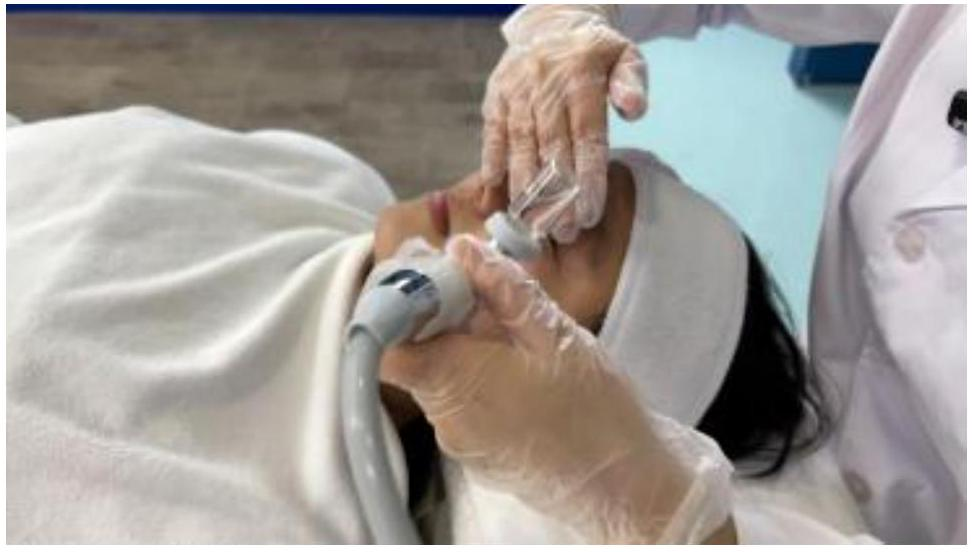
\includegraphics[max width=\textwidth, alt={}, center]{62504995-9f9b-47e6-9021-a213c68ce0b6-31_552_972_1644_1046}

\subsubsection{Maniglia a vibrazione ultrasonica}
Si consiglia di utilizzare lo spray caldo per 5 minuti per aprire i pori. Cliccare sull'icona della vibrazione ultrasonica, scegliere la modalità continua e impostare l'intensità da 5. Procedere delicatamente verso l'alto in base alla consistenza della pelle.\\

\includegraphics[max width=\textwidth, alt={}, center]{62504995-9f9b-47e6-9021-a213c68ce0b6-32_543_962_255_1046}

\begin{itemize}
  \item Il manico vibrante a ultrasuoni è adatto per pelli grasse e miste e può concentrarsi sulla zona T.
\end{itemize}

\subsubsection{Maniglia RF bipolare}
Selezionare la funzione RF bipolare, selezionare la modalità continua, regolare l'energia (intensità), impostare l'energia da 5.

Applicare il gel uniformemente sul viso, fare clic su Avvia, in base alla consistenza della pelle sollevando verso l'alto, il tempo di funzionamento è si consigliano 15-20 minuti.\\
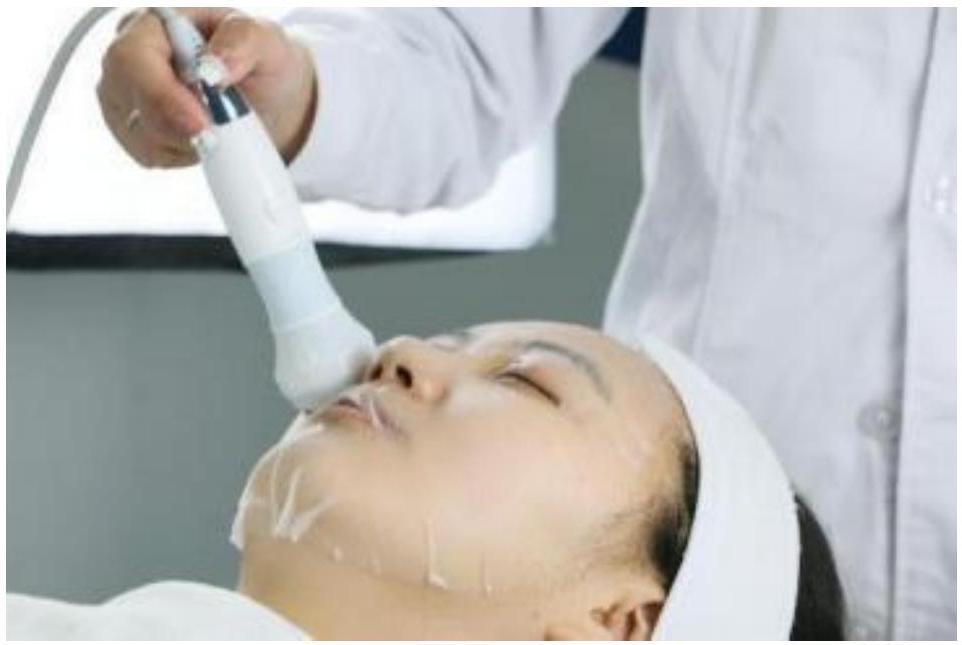
\includegraphics[max width=\textwidth, alt={}, center]{62504995-9f9b-47e6-9021-a213c68ce0b6-32_645_962_1032_1046}

\subsubsection{Maniglia microcorrente bipolare}
Selezionare la funzione microcorrente bipolare, selezionare Modalità continua, impostare l'energia (intensità) da 2 per gli occhi. Applicare uniformemente il gel freddo sul viso, in base alla consistenza della pelle, sollevando verso l'alto per 8-10 minuti. minuti.\\
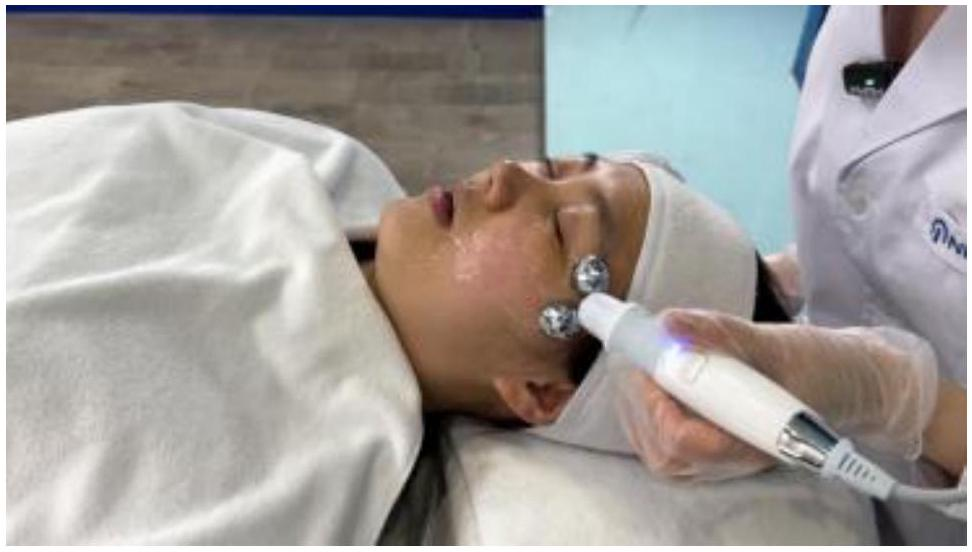
\includegraphics[max width=\textwidth, alt={}, center]{62504995-9f9b-47e6-9021-a213c68ce0b6-32_552_972_1795_1046}

\subsubsection{Manipolo multi-microcorrente}
Selezionare la funzione multi-microcorrente, selezionare la modalità continua, impostare l'energia (intensità) su 3 per guance, fronte e collo. Applicare uniformemente il gel freddo sul viso, in base alla grana della pelle, sollevando il viso per 8-10 minuti.\\
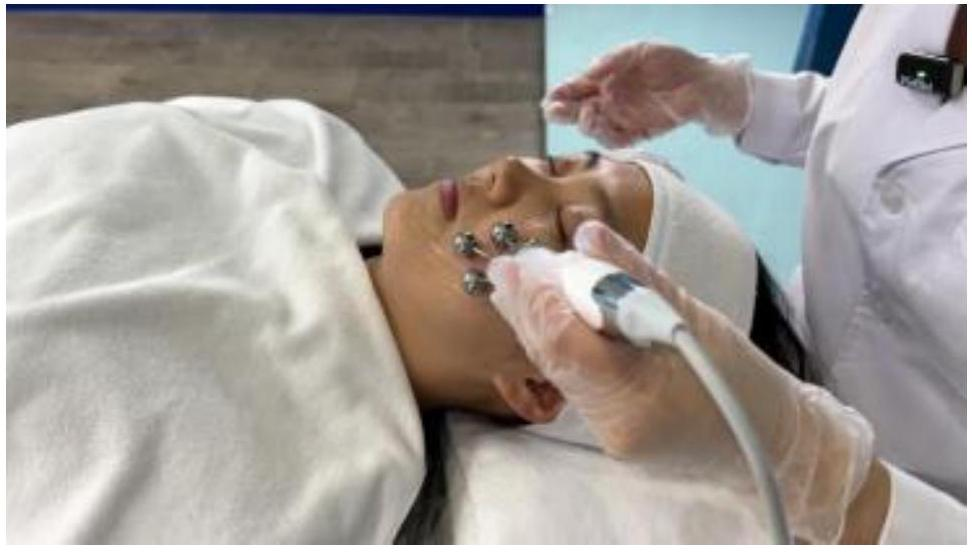
\includegraphics[max width=\textwidth, alt={}, center]{62504995-9f9b-47e6-9021-a213c68ce0b6-33_552_972_255_1046}

Selezionare la funzione ultrasuoni, scegliere la modalità continua, regolare l'intensità da 5, fare clic su Avvia, applicare l'essenza uniformemente sul viso, in base alla consistenza della pelle, dal basso verso l'alto con movimenti circolari.

\begin{figure}[H]
\begin{center}
\captionsetup{labelformat=empty}
\caption{5.2.8 Gestione dell'importazione degli ultrasuoni}
  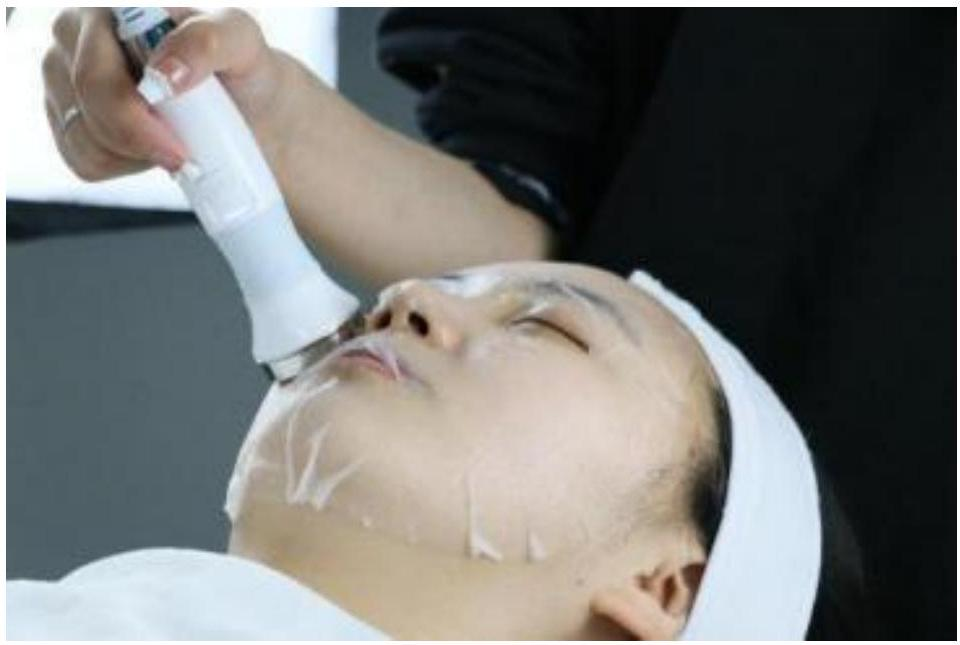
\includegraphics[alt={},max width=\textwidth]{62504995-9f9b-47e6-9021-a213c68ce0b6-33_645_960_920_1046}
\end{center}
\end{figure}

\subsubsection{Maniglia a martello freddo}
Selezionare la funzione martello freddo, regolare il freddo funzione o funzione calda a seconda della pelle. Per la funzione fredda, impostare l'intensità da 0 , fare clic su avvia, applicare un gel freddo o un prodotto calmante sulla zona da trattare, operare dal basso verso l'alto in un cerchio in base alla consistenza della pelle. Per la funzione calda, impostare l'intensità da 6 , regolare l'intensità in base alle esigenze del cliente tolleranza. Applicare il gel freddo sulla zona da trattare (o utilizzarlo durante l'applicazione della maschera), in base alla consistenza della pelle, sollevandola dal basso verso l'alto.\\

\includegraphics[max width=\textwidth, alt={}, center]{62504995-9f9b-47e6-9021-a213c68ce0b6-33_645_960_1683_1046}

AVVISO:Lo strumento deve essere pulito ogni volta dopo aver utilizzato la funzione di pulizia del viso. Per le modalità di pulizia, fare riferimento alle operazioni sopra descritte.

\subsection{Dopo il trattamento}
Applicare la pellicola medica per la riparazione dei traumi per 15 minuti/il gel medico per la riparazione dei traumi per 15 minuti, quindi rimuovere la pellicola per pulire, prendersi cura della pelle e proteggersi dal sole.

Suggerire ai clienti di utilizzare a casa una soluzione/crema per la riparazione dei traumi medici.

\subsection{Tabù}
\begin{itemize}
  \item Adatto a qualsiasi pubblico
  \item Soprattutto nelle aree con un inquinamento atmosferico persistente e grave
  \item Problemi della pelle come pelle spenta, stanchezza, pori ostruiti, strato corneo spesso, ecc.
  \item Acne, pelle acneica
\end{itemize}

\subsection{Questioni che richiedono attenzione}
\begin{itemize}
  \item Per chi ha uno strato corneo sottile o gravi striature rosse sugli zigomi, è vietato utilizzare la dermoabrasione, la radiofrequenza e la spalatura.
  \item Non utilizzare prodotti irritanti per la pelle o cosmetici entro 24 ore dal trattamento, prestare attenzione al sole protezione.
  \item Chi ha ferite non può operare per evitare infezioni.
  \item Disabili per persone con malattie della pelle.
\end{itemize}

\section{Manutenzione della macchina}
Per garantire un funzionamento sicuro e affidabile, la manutenzione regolare e la cura adeguata sono fondamentali. Questa sezione descrive la manutenzione ordinaria e periodica di questo sistema di movimentazione della macchina che gli operatori possono eseguire.

\subsection{Pulizia generale}
Pulire regolarmente l'esterno del dispositivo con un panno morbido e umido o in microfibra. È possibile utilizzare anche detergenti neutri e salviette senza alcol. La testina di comando dell'impugnatura deve essere pulita regolarmente dopo l'uso.

Si consiglia di pulire la testina una volta alla settimana o dopo l'uso. La testina di lavoro deve essere sempre priva di sporco e accessori.

\subsection{Trasporto, stoccaggio e movimentazione}
\begin{itemize}
  \item Ridurre al minimo il trasporto, perché il rischio di danni alle apparecchiature è maggiore.
  \item In caso di trasloco o stoccaggio, conservare e utilizzare l'imballaggio originale.
  \item Se ci si sposta in un'altra sala di trattamento, tenere il dispositivo in piano durante lo spostamento.
  \item Prestare attenzione durante la conservazione e l'uso, evitando urti, collisioni, schiacciamenti e vibrazioni.
\end{itemize}

Dopo ogni utilizzo, la macchina deve essere ripristinata e conservata in un luogo protetto dalla polvere.

\begin{itemize}
  \item In caso di spostamento o conservazione, conservare e utilizzare l'imballaggio originale. Non spostare il dispositivo a meno che necessario. Se ci si sposta in un'altra sala per trattamenti, tenerlo in piano durante il trasporto.
\end{itemize}

\subsection{Guida alla risoluzione dei problemi}
Questa sezione descrive i passaggi più basilari per la risoluzione dei problemi della macchina.

\subsubsection{La macchina non si avvia}
Zontrollare che l'alimentatore sia alimentato e che le spine di collegamento siano inserite saldamente da entrambe le estremità e La presa è accesa.

\begin{itemize}
  \item Verificare che il pulsante rosso di emergenza sia rilasciato.
\end{itemize}

\subsubsection{La testa operativa non funziona quando si preme il pulsante}
\begin{itemize}
  \item Verificare che la macchina sia in condizioni di funzionamento corrette.
  \item Controllare se il cavo e la spina di collegamento sono danneggiati, se qualche parte è danneggiata, contattare noi per sostituirci.
\end{itemize}

\subsubsection{Toccando la macchina si può verificare una scossa elettrica}
\begin{itemize}
  \item È necessario utilizzare tre spine di messa a terra e la presa di corrente deve essere adeguatamente collegata a terra.
  \item La tensione è instabile e dovrebbe essere introdotto un regolatore di tensione
\end{itemize}

\newpage

% --- INIZIO INFORMATIVA PRIVACY ---
\newpage

\section{INFORMATIVA PRIVACY}
\begin{center}
	(ai sensi dell'art. 13 del Regolamento UE 2016/679)
\end{center}

La presente informativa è resa ai sensi del Regolamento Generale sulla Protezione dei Dati (GDPR) e riguarda il trattamento dei dati personali dei clienti che si sottopongono a trattamenti e tecnologie estetiche.

\subsection*{Titolare del trattamento}

Il Titolare del trattamento è:

\begin{itemize}
	\item Denominazione centro estetico: \underline{\hspace{5cm}}
	\item Sede legale: \underline{\hspace{7cm}}
	\item P. IVA / C.F.: \underline{\hspace{6cm}}
	\item Contatti (telefono/email): \underline{\hspace{5cm}}
\end{itemize}

\subsection*{Tipologia di dati trattati}

Il Titolare può raccogliere e trattare le seguenti categorie di dati:

\begin{itemize}
	\item Dati anagrafici (nome, cognome, data di nascita)
	\item Dati di contatto (telefono, e-mail)
	\item Dati fiscali per eventuale fatturazione
	\item Dati particolari relativi allo stato di salute (allergie, patologie, gravidanza, terapie in corso) necessari per valutare l'idoneità ai trattamenti estetici
	\item Eventuali immagini fotografiche prima/dopo trattamento (previo consenso specifico)
\end{itemize}

\subsection*{Finalità del trattamento}

I dati personali sono trattati per le seguenti finalità:

\begin{enumerate}
	\item Esecuzione di trattamenti estetici e utilizzo di tecnologie professionali (laser, radiofrequenza, ultrasuoni, pressoterapia, ecc.)
	\item Valutazione dell'idoneità al trattamento
	\item Adempimenti amministrativi, contabili e fiscali
	\item Gestione degli appuntamenti
	\item Eventuale invio di comunicazioni promozionali (solo previo consenso separato)
	\item Eventuale utilizzo di immagini per finalità informative o promozionali (solo previo consenso separato)
\end{enumerate}

\subsection*{Base giuridica del trattamento}

Il trattamento dei dati si fonda su:

\begin{itemize}
	\item Esecuzione del contratto/prestazione richiesta
	\item Adempimento di obblighi di legge
	\item Consenso esplicito dell'interessato per il trattamento di dati particolari (sanitari)
	\item Consenso separato per marketing e utilizzo immagini
\end{itemize}

\subsection*{Modalità di trattamento}

Il trattamento dei dati avviene mediante strumenti cartacei e/o informatici, nel rispetto dei principi di correttezza, liceità, trasparenza e tutela della riservatezza.

Sono adottate adeguate misure di sicurezza per prevenire accessi non autorizzati, perdita o diffusione dei dati.

\subsection*{Conservazione dei dati}

I dati personali saranno conservati:

\begin{itemize}
	\item Per il tempo necessario all'erogazione del servizio
	\item Per il periodo previsto dalla normativa fiscale e civilistica
	\item Fino a revoca del consenso per finalità di marketing o utilizzo immagini
\end{itemize}

\subsection*{Comunicazione dei dati}

I dati potranno essere comunicati a:

\begin{itemize}
	\item Consulenti fiscali e amministrativi
	\item Software gestionali utilizzati per la gestione clienti
	\item Autorità competenti, ove previsto dalla legge
\end{itemize}

I dati non saranno diffusi senza consenso.

\subsection*{Diritti dell'interessato}

L'interessato può esercitare in qualsiasi momento i seguenti diritti:

\begin{itemize}
	\item Accesso ai propri dati
	\item Rettifica o aggiornamento
	\item Cancellazione (diritto all'oblio)
	\item Limitazione del trattamento
	\item Opposizione al trattamento
	\item Revoca del consenso
	\item Reclamo all'Autorità Garante per la Protezione dei Dati Personali
\end{itemize}

Le richieste possono essere inviate ai recapiti del Titolare sopra indicati.

\subsection*{Natura del conferimento dei dati}

Il conferimento dei dati è necessario per l'erogazione dei trattamenti estetici.
Il mancato conferimento può comportare l'impossibilità di eseguire il servizio.

\subsection*{CONSENSO}

Il/La sottoscritto/a dichiara di aver ricevuto e compreso la presente informativa.

\vspace{0.8cm}

Data: \underline{\hspace{5cm}} 

\vspace{15pt}
Firma: \underline{\hspace{6cm}}

\vspace{1cm}

$\square$ Acconsento al trattamento dei dati particolari (sanitari)

\vspace{0.3cm}
$\square$ Acconsento all'utilizzo delle immagini per finalità promozionali

\vspace{0.3cm}
$\square$ Acconsento a ricevere comunicazioni promozionali

% --- FINE INFORMATIVA PRIVACY ---

\newpage


\begin{figure}[H]
	\centering
	\includegraphics[width=0.7\paperwidth,height=\paperheight, keepaspectratio]{"../cose da aggiungere/privacy_conformita/dichiarazione_conformita"}
\end{figure}


\section{Simboli}
\begin{figure}[H]
	\centering
	
\includegraphics[width=\linewidth]{pittogrammi_1}
%	\caption{}
	\label{fig:pittogrammi1}
\end{figure}
\begin{figure}[H]
	\centering
	
\includegraphics[width=\linewidth]{pittogrammi_2}
%	\caption{}
	\label{fig:pittogrammi2}
\end{figure}
\begin{figure}[H]
	\centering
	
\includegraphics[width=\linewidth]{pittogrammi_3}
%	\caption{}
	\label{fig:pittogrammi3}
\end{figure}
\begin{figure}[H]
	\centering
	
\includegraphics[width=\linewidth]{pittogrammi_4}
%	\caption{}
	\label{fig:pittogrammi4}
\end{figure}
\begin{figure}[H]
	\centering
	
\includegraphics[width=\linewidth]{pittogrammi_5}
%	\caption{}
	\label{fig:pittogrammi5}
\end{figure}



\end{document}